\documentclass[11pt,a4paper]{article}
\usepackage[margin=2cm]{geometry}
\usepackage{amsmath,amssymb}
\usepackage{booktabs,longtable,float,graphicx,enumitem}
\usepackage[table]{xcolor}
\usepackage{tikz}
\usetikzlibrary{arrows.meta,positioning,fit,backgrounds}
\usepackage{listings}
\usepackage{microtype}
\usepackage[hidelinks]{hyperref}
\lstset{basicstyle=\ttfamily\scriptsize,breaklines=true,columns=fullflexible,frame=single,keepspaces=true}
\setlength{\parindent}{0pt}
\setlength{\parskip}{4pt}

% ---- edit before submitting -------------------------------------------------
\newcommand{\studentname}{Erik Mirzoyan}
\newcommand{\repourl}{https://github.com/10mirzoyan71/photonicsai-hw3}
% -----------------------------------------------------------------------------
\newcommand{\todobox}[1]{\begin{center}\fcolorbox{red}{red!5}{\begin{minipage}{0.92\linewidth}#1\end{minipage}}\end{center}}

\begin{document}
\begin{center}
{\Large\bfseries PhotonicsAI --- AI-Driven Science and Autonomous Laboratories}\\[3pt]
{\large Homework 3: Hardware in the Loop}\\[6pt]
Name: \studentname\\[2pt]
Code: \url{\repourl}
\end{center}

\textbf{Instrument:} one of the lab cameras, a \textbf{Hikrobot MV-CS028-10UM} industrial camera (monochrome, USB~3.0,
USB3~Vision\,/\,GenICam). \textbf{Interface:} Hikrobot's MVS SDK (the \texttt{MvCameraControl} library, used through the Python
interface that MVS installs; MVS~5.1.0, camera SDK~4.8.2.2).
The code: \texttt{camera/} (the connector), \texttt{mcp\_server/} (the MCP server), \texttt{agent/} (the agent system with the
hardware turn), \texttt{tests/}.

\textbf{Project.} The agent system turns the lab camera into a characterised measuring instrument on its own, from a
plain-language request: it finds working settings (exposure without saturation, free of the room lights' flicker),
measures the camera's noise model (conversion gain, read noise, full well, dark level) and its stability, and then puts
these measured numbers into the camera model of the Homework~2 focusing bench to predict the focusing enhancement that a
wavefront-shaping experiment would reach with this camera. The lab has no laser for this homework, so the scene is a white
surface under the room lights; the lab's DMDs with this camera would be the next step towards running the Homework~2
experiment on real hardware.

%======================================================================
\section*{(a) The connector}
%======================================================================
\texttt{camera/base.py} defines the interface every camera implements: \texttt{info()}, \texttt{set\_exposure(us)},
\texttt{set\_gain(dB)}, \texttt{set\_roi(x, y, w, h)}, \texttt{grab()} (one frame as a \texttt{uint16} array) and
\texttt{close()}. \texttt{camera/hikrobot\_camera.py} implements it with the MVS SDK:
\begin{center}\small
\begin{tabular}{@{}ll@{}}
\toprule connector method & MVS SDK call / camera feature (GenICam name)\\ \midrule
open & \texttt{MV\_CC\_EnumDevices} $\to$ \texttt{MV\_CC\_CreateHandle} $\to$ \texttt{MV\_CC\_OpenDevice} (exclusive)\\
setup & \texttt{ExposureAuto}=Off, \texttt{GainAuto}=Off, \texttt{ADCBitDepth}=deepest (12 bit), \texttt{BlackLevel}=180,\\
 & \texttt{PixelFormat}=Mono12 (else Mono10, Mono8), \texttt{TriggerMode}=On, \texttt{TriggerSource}=Software,\\
 & \texttt{MV\_CC\_StartGrabbing}\\
\texttt{set\_exposure} / \texttt{set\_gain} & \texttt{ExposureTime} [\textmu s] / \texttt{Gain} [dB] (float features, value read back)\\
\texttt{set\_roi} & \texttt{OffsetX}, \texttt{OffsetY}, \texttt{Width}, \texttt{Height} (camera increments; acquisition stopped)\\
\texttt{grab} & \texttt{TriggerSoftware} $\to$ \texttt{MV\_CC\_GetImageBuffer} $\to$ copy $\to$ \texttt{MV\_CC\_FreeImageBuffer}\\
\texttt{info} & \texttt{WidthMax}, \texttt{HeightMax}, ranges of \texttt{ExposureTime} and \texttt{Gain}, current settings\\
\bottomrule
\end{tabular}
\end{center}
With the software trigger every frame is exposed after the command that precedes it, with the settings just applied, so
a measurement can never come from a stale frame. Sensor size, bit depth and ranges are read from the camera, not assumed.
\texttt{camera/sim\_camera.py} implements the same interface with a simulated 12-bit camera (shot noise, read noise, dark
current, fixed-pattern noise, saturation, a slowly drifting light source) looking at a laser speckle pattern
(\texttt{sim}) or at a white surface under room lights that flicker at 100\,Hz (\texttt{sim-room}; a frame integrates the
flicker from a random phase, so its mean fluctuates unless the exposure spans whole 10\,ms periods). It is used for the
tests and for the dry runs below; a photon-transfer measurement on it recovers its conversion gain (2.38 vs.\ 2.40
e$^-$/DN) and read noise (5.97 vs.\ 6.0\,e$^-$), which checks that the analysis the agent uses is sound.

\textbf{Check of the SDK on the laptop (without the camera):} \texttt{tests/check\_mvs\_sdk.py} loads the MVS library and
checks every function, structure, field and pixel-format code the connector uses: all present (camera SDK 4.8.2.2).
\textbf{Connection test with the camera plugged in} (\texttt{tests/check\_real\_camera.py}; logs in
\texttt{tests/real\_camera\_check/}): the connector opened the camera through the SDK and read back the model
(MV-CS028-10UM, USB3 Vision), the sensor (1936\,$\times$\,1464), the pixel format (Mono12) and the ranges (exposure
9\,$\mu$s--10\,s, gain 0--24\,dB). Two settings of the camera itself were wrong for measurements, and the test found
both: the camera digitised with 8 bits (\texttt{ADCBitDepth\_8}), so the Mono12 values came in steps of 17\,DN; and the
default \texttt{BlackLevel} put the dark level at 0\,DN, which cut off the negative half of the dark noise (half of the
dark pixels read exactly 0). The connector now selects the deepest ADC mode (\texttt{ADCBitDepth\_12}) and sets
\texttt{BlackLevel} so that the dark level sits about 60\,DN above zero. With these settings, looking at a white wall at
0\,dB: mean 819.7\,DN at 2\,ms and 1575.0\,DN at 4\,ms, i.e.\ the signal above the dark level doubles (ratio 2.00);
42\,frames/s with the software trigger at 4\,ms; a 256\,$\times$\,256 ROI and the return to the full sensor work; with
the camera covered, the dark level is 62.4\,DN and the temporal noise 0.95\,DN rms.

%======================================================================
\section*{(b) The MCP server}
%======================================================================
\texttt{mcp\_server/camera\_server.py} is an MCP server (Python MCP SDK, \texttt{FastMCP}, stdio transport). It opens the
camera through the connector (\texttt{CAMERA\_KIND=hikrobot} for the lab camera, \texttt{sim} or \texttt{sim-room} for the
simulated one) and
carries out every tool call with it. Each tool is one action of the camera or one reading it returns; the list below is the
server's own \texttt{list\_tools}:
{\small% generated by agent/render_tools.py from the server's list_tools
\begin{longtable}{@{}l p{0.3\linewidth} p{0.45\linewidth}@{}}
\toprule tool & arguments & what it does\\ \midrule \endhead
\texttt{camera\_info} & -- & Describe the camera: vendor, model, sensor size, bit depth (max DN), exposure and gain ranges, the lab limits, and the current settings (exposure, gain, ROI).\\
\texttt{set\_exposure} & exposure\_us: number & Set the exposure time in microseconds.\\
\texttt{set\_gain} & gain\_db: number & Set the analog gain in dB.\\
\texttt{set\_roi} & x: integer, y: integer, width: integer, height: integer & Set the region of interest: offset (x, y) and size in sensor pixels.\\
\texttt{reset\_roi} & -- & Use the full sensor again.\\
\texttt{set\_illumination} & level: number & Light source level 0..1 on the simulated camera only (0 = dark, for dark frames).\\
\texttt{capture} & n\_frames: integer (opt.), label: string (opt.), regions: array (opt.) & Acquire n\_frames frames with the current settings and save them.\\
\texttt{capture\_series} & n\_frames: integer, interval\_s: number, label: string (opt.), regions: array (opt.) & Stability measurement: n\_frames frames, one every interval\_s seconds, with the current settings.\\
\texttt{analyze\_frame} & frame\_file: string, black\_level\_dn: number (opt.), region: object (opt.) & Speckle and beam measures of a saved frame (first frame of the file): speckle contrast and grain size (FWHM of the intensity autocorrelation) inside `region` (or the whole frame), and the beam centroid and D4sigma widths.\\
\bottomrule
\end{longtable}
}
Every tool returns \texttt{ok} and its result, or \texttt{ok=false} and the reason (out of the camera's range, above a
lab limit, device error), so a refused command reaches the agent instead of crashing the run. The lab limits (maximum
exposure, gain, frames, series length) are set when the server starts. Every call is appended to \texttt{calls.jsonl}
(time, tool, arguments, result): this file is the record of what the instrument did, and the tables and sequence diagrams
in (f) are generated from it. Frames are saved as \texttt{.npy} with a preview \texttt{.png}.

%======================================================================
\section*{(c) One agent holds the tools}
%======================================================================
The roles are those of Homeworks 1 and 2: orchestrator, scientist, general agent, executor, plus the human stop. Only the
\textbf{executor} receives the MCP server: \texttt{agent/mcp\_bridge.py} starts the server, keeps one MCP session open for
the whole run (so the camera keeps its settings between calls) and gives the executor the server's tools with the schemas
the server publishes. No other role can reach the camera.
The decision to call a tool is a model call: at each step of a hardware turn the executor's model reads the dialogue
(the request, the scientist's plan, every earlier command and measurement) and returns a structured decision
\texttt{HWDecision(action, command, command\_args, n\_frames, label, regions, analyze, black\_level\_dn,
analysis\_region, question, summary, reason)}, where
\texttt{action} is \emph{command} (one command tool, then a capture), \emph{measure}, \emph{ask\_person} or \emph{finish}.
The graph then makes exactly that MCP call. The executor also keeps its software tools from the earlier homeworks: the
coding tool (scripts that analyse the saved frames) and the focusing tool of the Homework~2 simulated bench, whose camera
model (read noise, full well, signal level, light-source noise) can be set per experiment from the real camera's
measured numbers.

%======================================================================
\section*{(d) Hardware in the loop}
%======================================================================
The hardware turn is built like the human stop of Homework~2: the orchestrator's decision (a model call) can choose a new
destination, \texttt{hardware}, when the next step needs the instrument. The graph then gives the turn to the executor in a
loop of nodes:
\begin{center}
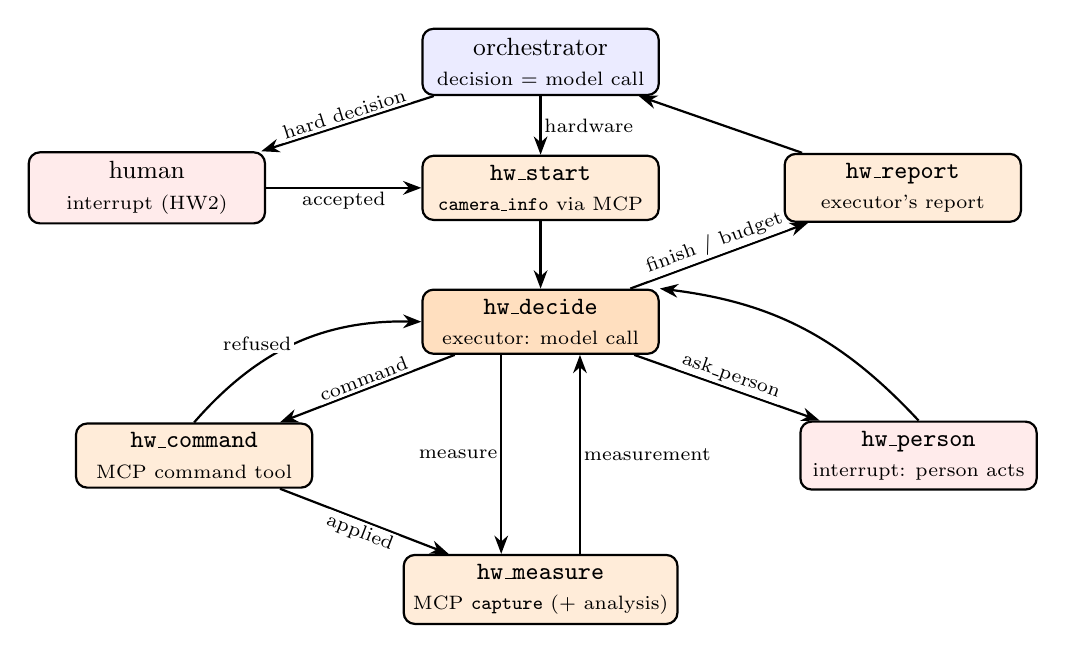
\begin{tikzpicture}[>=Stealth, font=\small,
  n/.style={draw,thick,rounded corners,minimum width=30mm,minimum height=8mm,align=center},
  e/.style={->,thick}, l/.style={font=\scriptsize,fill=white,inner sep=1pt}]
  \node[n,fill=blue!8] (o) at (0,0) {orchestrator\\\scriptsize decision = model call};
  \node[n,fill=red!8] (h) at (-5,-1.6) {human\\\scriptsize interrupt (HW2)};
  \node[n,fill=orange!15] (s) at (0,-1.6) {\texttt{hw\_start}\\\scriptsize \texttt{camera\_info} via MCP};
  \node[n,fill=orange!25] (d) at (0,-3.3) {\texttt{hw\_decide}\\\scriptsize executor: model call};
  \node[n,fill=orange!15] (c) at (-4.4,-5.0) {\texttt{hw\_command}\\\scriptsize MCP command tool};
  \node[n,fill=orange!15] (m) at (0,-6.7) {\texttt{hw\_measure}\\\scriptsize MCP \texttt{capture} (+ analysis)};
  \node[n,fill=red!8] (p) at (4.8,-5.0) {\texttt{hw\_person}\\\scriptsize interrupt: person acts};
  \node[n,fill=orange!15] (r) at (4.6,-1.6) {\texttt{hw\_report}\\\scriptsize executor's report};
  \draw[e] (o) -- node[l,right]{hardware} (s);
  \draw[e] (o) -- node[l,above,sloped]{hard decision} (h);
  \draw[e] (h) -- node[l,below]{accepted} (s);
  \draw[e] (s) -- (d);
  \draw[e] (d) -- node[l,above,sloped]{command} (c);
  \draw[e] (c) -- node[l,below,sloped]{applied} (m);
  \draw[e] (c.north) to[bend left=25] node[l,left]{refused} (d.west);
  \draw[e] ([xshift=-5mm]d.south) -- node[l,left]{measure} ([xshift=-5mm]m.north);
  \draw[e] ([xshift=5mm]m.north) -- node[l,right]{measurement} ([xshift=5mm]d.south);
  \draw[e] (d) -- node[l,above,sloped]{ask\_person} (p);
  \draw[e] (p.north) to[bend right=20] (d.north east);
  \draw[e] (d) -- node[l,above,sloped]{finish / budget} (r);
  \draw[e] (r) -- (o);
\end{tikzpicture}
\end{center}
Every node writes one turn into the dialogue: the instrument's reply to a command (the value it applied, or why it refused)
and every measurement (frame statistics, temporal noise, region values, speckle/beam measures, file name). The next
\texttt{hw\_decide} reads those turns before it chooses again: \emph{decide $\to$ command the hardware $\to$ receive the
measurement $\to$ decide again}. A refused command goes straight back to \texttt{hw\_decide}. The turn ends when the
executor chooses \emph{finish} (or after 12 steps); \texttt{hw\_report} then writes the settings and measurements the
camera returned, marked VERIFIED, and the turn returns to the orchestrator, which may finish only after such a record exists.
The human stop stays: a hardware turn that changes settings or runs a long acquisition is a hard decision for which the
orchestrator may ask the person first (accepted $\to$ the turn runs; refused $\to$ it does not, and a record says so), and
inside the turn \emph{ask\_person} pauses the graph for what only a person can do, e.g.\ block the light for dark frames on
the lab bench, where the light is not under software control. Both stops are LangGraph interrupts on a checkpointed thread.

%======================================================================
\section*{(e) Architecture of the system so far}
%======================================================================
\begin{center}
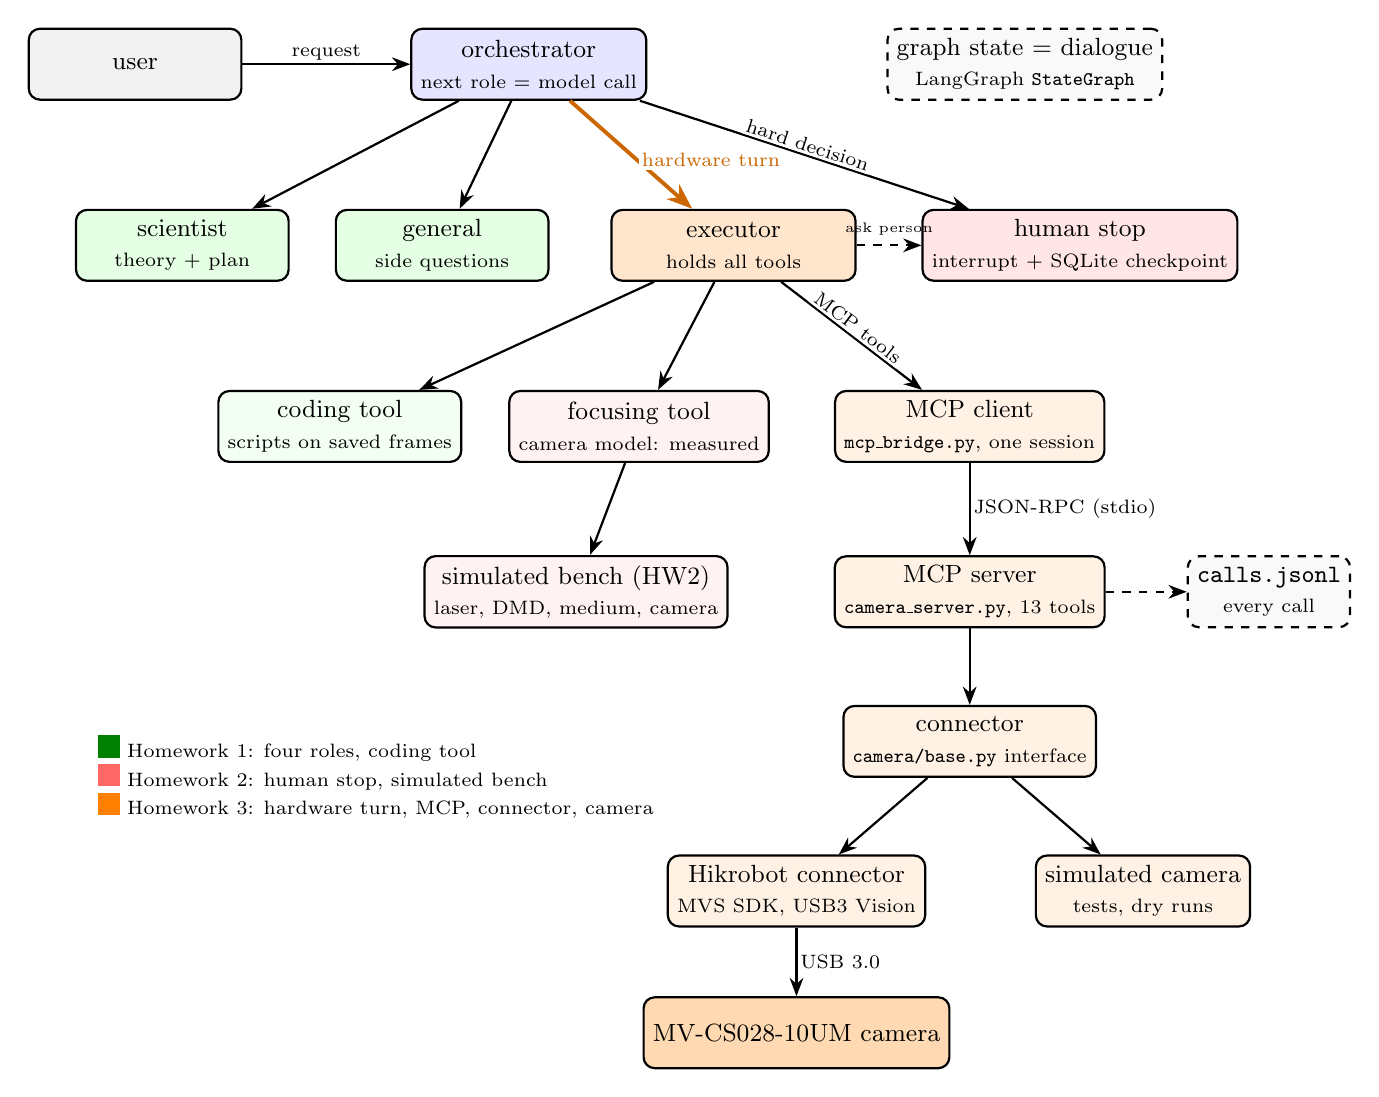
\begin{tikzpicture}[>=Stealth, font=\small,
  b/.style={draw,thick,rounded corners,minimum width=27mm,minimum height=9mm,align=center},
  e/.style={->,thick}, l/.style={font=\scriptsize,fill=white,inner sep=1pt}]
  \node[b,fill=gray!10] (u) at (0,0) {user};
  \node[b,fill=blue!10] (o) at (5,0) {orchestrator\\\scriptsize next role = model call};
  \node[b,fill=gray!5,dashed] (st) at (11.3,0) {graph state = dialogue\\\scriptsize LangGraph \texttt{StateGraph}};
  \node[b,fill=green!10] (sc) at (0.6,-2.3) {scientist\\\scriptsize theory + plan};
  \node[b,fill=green!10] (g) at (3.9,-2.3) {general\\\scriptsize side questions};
  \node[b,fill=orange!20,minimum width=31mm] (ex) at (7.6,-2.3) {executor\\\scriptsize holds all tools};
  \node[b,fill=red!10] (h) at (12.0,-2.3) {human stop\\\scriptsize interrupt + SQLite checkpoint};
  \node[b,fill=green!5] (ct) at (2.6,-4.6) {coding tool\\\scriptsize scripts on saved frames};
  \node[b,fill=red!5] (ft) at (6.4,-4.6) {focusing tool\\\scriptsize camera model: measured};
  \node[b,fill=red!5] (bench) at (5.6,-6.7) {simulated bench (HW2)\\\scriptsize laser, DMD, medium, camera};
  \node[b,fill=orange!10] (mc) at (10.6,-4.6) {MCP client\\\scriptsize \texttt{mcp\_bridge.py}, one session};
  \node[b,fill=orange!10] (ms) at (10.6,-6.7) {MCP server\\\scriptsize \texttt{camera\_server.py}, 13 tools};
  \node[b,fill=orange!10] (cn) at (10.6,-8.6) {connector\\\scriptsize \texttt{camera/base.py} interface};
  \node[b,fill=orange!10] (hk) at (8.4,-10.5) {Hikrobot connector\\\scriptsize MVS SDK, USB3 Vision};
  \node[b,fill=orange!10] (sm) at (12.8,-10.5) {simulated camera\\\scriptsize tests, dry runs};
  \node[b,fill=orange!30] (cam) at (8.4,-12.3) {MV-CS028-10UM camera};
  \draw[e] (u) -- node[l,above]{request} (o);
  \draw[e] (o) -- (sc); \draw[e] (o) -- (g);
  \draw[e,orange!80!black,line width=1.4pt] (o) -- node[l,right,pos=0.55]{hardware turn} (ex);
  \draw[e] (o) -- node[l,above,sloped]{hard decision} (h);
  \draw[e,dashed] (ex.east) -- node[above,font=\tiny]{ask person} (h.west);
  \draw[e] (ex) -- (ct); \draw[e] (ex) -- (ft); \draw[e] (ex) -- node[l,above,sloped]{MCP tools} (mc);
  \draw[e] (ft) -- (bench);
  \draw[e] (mc) -- node[l,right]{JSON-RPC (stdio)} (ms);
  \draw[e] (ms) -- (cn); \draw[e] (cn) -- (hk); \draw[e] (cn) -- (sm);
  \draw[e] (hk) -- node[l,right]{USB 3.0} (cam);
  \node[b,fill=gray!5,dashed,minimum width=20mm] (log) at (14.4,-6.7) {\texttt{calls.jsonl}\\\scriptsize every call};
  \draw[e,dashed] (ms) -- (log);
  \node[font=\scriptsize,align=left,anchor=north west] at (-0.6,-8.4) {%
    \textcolor{green!50!black}{\rule{8pt}{8pt}} Homework 1: four roles, coding tool\\
    \textcolor{red!60}{\rule{8pt}{8pt}} Homework 2: human stop, simulated bench\\
    \textcolor{orange}{\rule{8pt}{8pt}} Homework 3: hardware turn, MCP, connector, camera};
\end{tikzpicture}
\end{center}
The scientist, the general agent and the human answer the orchestrator, and every specialist turn returns to it; all turns
are written into the one dialogue that is the graph's state. Sequence diagrams of the runs are in (f), one per run.

%======================================================================
\section*{(f) Use cases and the demo}
%======================================================================
\textbf{Setup at the lab.} The MV-CS028-10UM on the laptop's USB~3 port, without a lens (a sheet of paper over the
sensor opening diffuses the light), looking at a white wall next to a window under LED room lights; no laser. Every run is
\texttt{python run\_hw3.py --camera hikrobot --thread <name> --request "..."} (Claude Sonnet~5.5 through the Claude Code
CLI); the lab limits were 500\,ms exposure, 24\,dB gain and 16 frames per capture. When the agent asked for something
only a person can do (block or unblock the light) or, with \texttt{--human}, for approval of a hard decision, the person at
the bench answered and the reply was passed to the run as given (in English). The tables, sequence diagrams and frames
below are generated from each run's \texttt{calls.jsonl} and transcript by \texttt{agent/render\_hw3.py}.

{\footnotesize{\footnotesize\begin{longtable}{@{}p{0.3\linewidth} r r r p{0.4\linewidth}@{}}
\toprule request & decisions & hw steps & MCP calls & verified result\\ \midrule \endhead
Set the camera so that the white surface uses most of the camera's range without saturating, and report the exposure and gain you chose. & 2 & 4 & 7 & 9400 us, 0 dB: max 3592 DN, 0 saturated px\\
The camera looks at a white surface under the lab's room lights, which may flicker. Find an exposure at which the frame-to-frame brightness is stable, with the image well exposed but not saturated, and report how strong the flicker is at a short exposure and at the exposure you chose. & 3 & 13 & 23 & 10000 us, 0 dB: max 2497 DN, 0 saturated px\\
At an exposure free of the light flicker, measure how stable the brightness is over two minutes and report the drift. & 4 & 8 & 11 & script drift\_analysis.py: SLOPE\_PCT\_PER\_MIN=-3.43, TOTAL\_CHANGE\_PCT=-6.859, FLICKER\_NFRAMES\_5ms=16, FLICKER\_MEAN\_DN\_5ms=1157\\
Measure this camera's read noise, conversion gain and full well capacity in electrons. Then use these measured numbers as the camera of the Homework 2 focusing bench and predict the focusing enhancement we can expect with this camera, choosing the bench signal level so that the focus does not saturate it. & 5 & 12 & 20 & focusing tool (simulated bench), experiment 4: enhancement 11\\
Set the gain to 12 dB and choose the exposure so that the wall is at about half of the camera's range, then report the exposure and the temporal noise. & 3 & 10 & 11 & 3250 us, 11.991 dB: max 2163 DN, 0 saturated px\\
Set the gain to 12 dB and choose the exposure so that the wall is at about half of the camera's range, then report the exposure and the temporal noise. & 3 & 3 & 6 & 4090 us, 11.991 dB: max 2201 DN, 0 saturated px\\
Do not use the camera. The lab camera (Hikrobot MV-CS028-10UM) was measured in an earlier run: conversion gain 6.14 e-/DN, read noise 5.78 e-, full well at least 24766 e-. With the focusing tool, compare the focusing enhancement at the Homework 2 settings (macropixel 4, focus\_size 3, bg\_inner 6, bg\_outer 20, bg\_regions 8, iterations 40000, flips 4, remeasure true) for the bench's default camera and for this measured camera, with the bench signal level chosen so that the focus does not saturate this camera. Report both enhancements. & 3 & 0 & 0 & focusing tool (simulated bench), experiment 4: enhancement 30.63\\
\bottomrule
\end{longtable}}
}
What the runs found:
\begin{itemize}[leftmargin=*,itemsep=1pt]
\item \textbf{Auto-exposure:} from a first frame at 4\,ms (peak 1587\,DN) the executor scaled the exposure to 9\,ms and then
9.4\,ms: peak 3592\,DN (87.7\,\% of full scale), no saturated pixel, gain left at 0\,dB.
\item \textbf{Flicker:} the LED lights hardly flicker. The frame-to-frame spread of the mean was 0.14\,\% at 1\,ms and
0.05\,\% at 10\,ms; the agent chose 10\,ms (one 100\,Hz period, 59\,\% of full scale) and stated that the flicker is weak.
\item \textbf{Stability:} 121 frames over 120\,s at 10\,ms: the brightness fell smoothly by 3.43\,\%/min (6.9\,\% in
total, residual scatter 0.14\,\%). The agent asked the person to block the light for the dark level (64.1\,DN) and
did not attribute the drift to the camera; with daylight from the window in the evening, the light itself was changing.
\item \textbf{Noise model and focusing prediction:} the person blocked and then unblocked the light when asked. From dark
frames and a photon-transfer series the agent measured a conversion gain of 6.14\,e$^-$/DN, a read noise of 5.78\,e$^-$ and
a full well of at least 24\,766\,e$^-$ (limited by the 12-bit ADC, so a lower bound). With these numbers as the bench's
camera and a signal level chosen so that the focus stays at about 66\,\% of the full well, the focusing tool predicted an
enhancement of 10.8 for the quick configuration the agent chose (64 segments, 6000 iterations). The agent itself noted
that this value is set by the bench configuration rather than by the camera; for binary-amplitude shaping with 64
segments the expected enhancement is about $N/2\pi \approx 10$. A follow-up run without the camera (use case~7) therefore
compared both cameras at the Homework~2 settings (256 segments, 40\,000 iterations, the same signal of 400\,e$^-$/px): the
bench's default camera gave 33.55 and the measured lab camera 30.63, about 9\,\% lower (at 100\,e$^-$/px: 26.45 and 25.12),
with no saturated pixel. One run per setting, so the run-to-run spread is not included.
\item \textbf{Human stops, first attempt:} the person approved the hardware turn. Inside it the agent asked for the light to
be blocked for dark frames; the person replied without blocking it (having not been told what the dark frames were for).
The agent did not trust the reply: it checked each ``dark'' set, saw that it was as bright as the wall (2054 vs.\
2076\,DN), asked again (three requests in all), and finally reported the dark level and read noise as undetermined
instead of using bright frames; the person approved its decision to finish. \textbf{Second run} (recorded): the orchestrator stopped twice for approval (before the hardware turn
and before finishing); the person answered \emph{yes} both times; result 4.09\,ms at 12\,dB, wall at 49.6\,\% of full
scale, temporal noise 35.9\,DN rms.
\end{itemize}

\begin{figure}[H]\centering
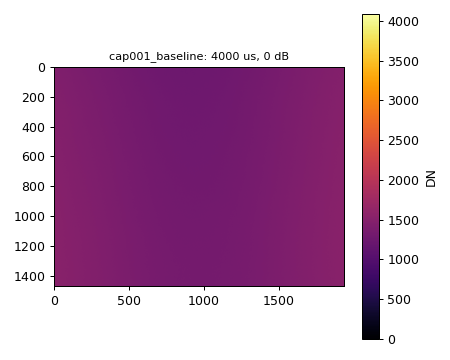
\includegraphics[width=0.32\linewidth]{runs/img/real_uc1_first_4ms.png}\hfill
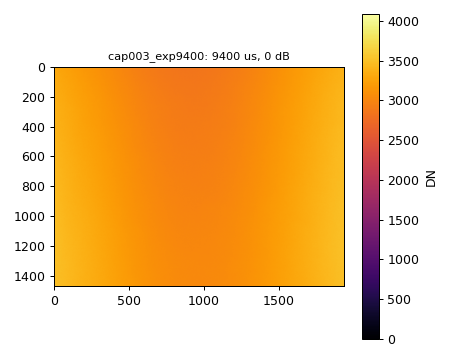
\includegraphics[width=0.32\linewidth]{runs/img/real_uc1_final_9400us.png}\hfill
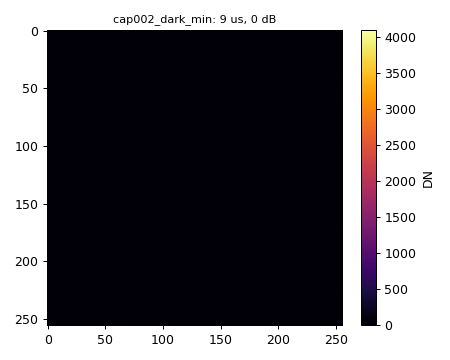
\includegraphics[width=0.32\linewidth]{runs/img/real_uc6_dark.png}\\[2pt]
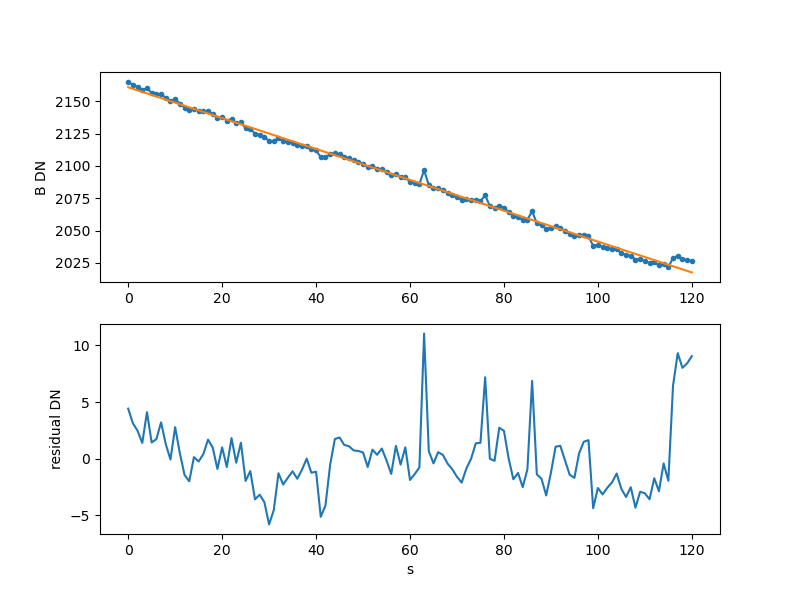
\includegraphics[width=0.36\linewidth]{runs/img/real_uc4_drift.png}\hfill
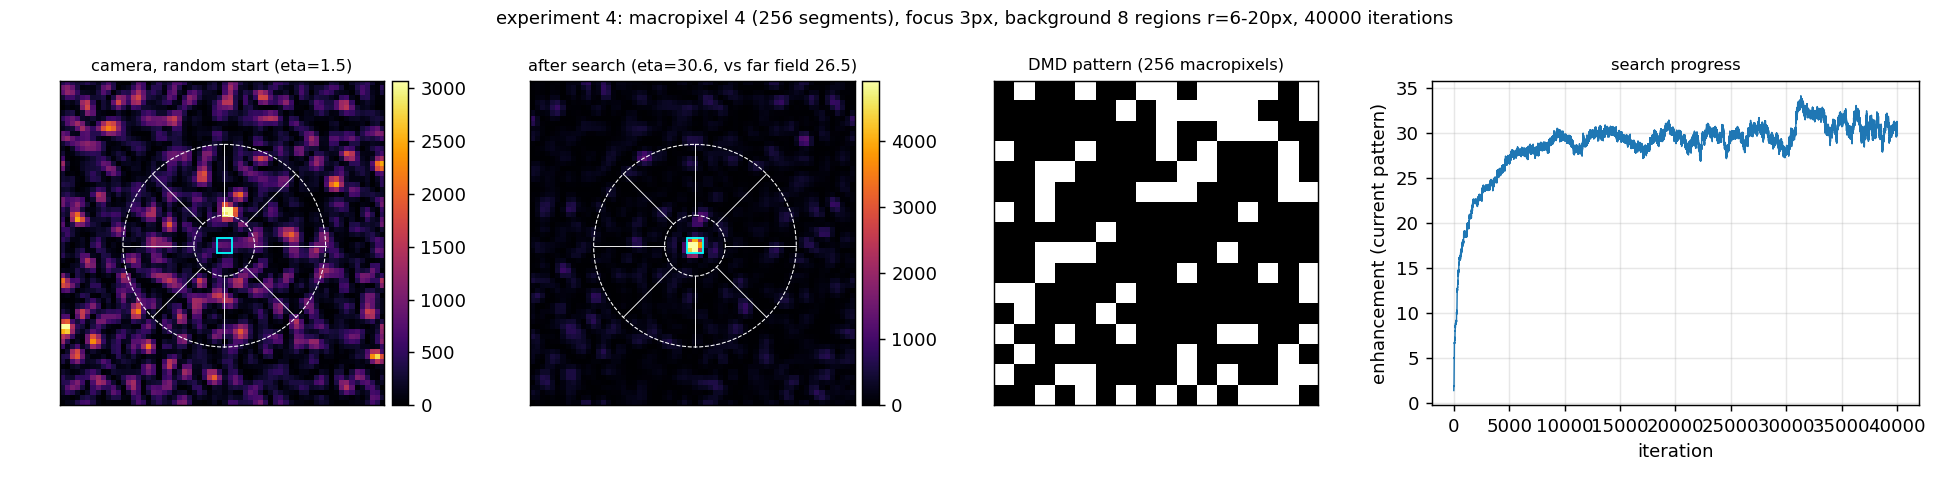
\includegraphics[width=0.62\linewidth]{runs/img/real_uc8_bench_measured_camera.png}
\caption{What the instrument returned (previews saved by the MCP server, 0--4095\,DN). Top: use case~1, the first frame at
4\,ms and the frame at the 9.4\,ms the agent chose (the white wall seen through the paper diffuser, brighter towards the
sides); use case~4, a dark frame taken after the person blocked the light. Bottom left: use case~3, the frame-mean
brightness over 120\,s and the residuals of the linear fit (the agent's analysis script). Bottom right: use case~7, the
Homework~2 bench with the measured camera model: speckle at the random start, the focus after 40\,000 iterations, the DMD
pattern and the search progress (simulation).}
\end{figure}

\textbf{Demo videos} (screen recordings, cropped to the live camera view and the run's terminal, no sound), in the
repository folder \texttt{video/} and attached to the email: \texttt{hw3\_demo\_real\_camera.mp4} (59\,s, use case~1: the
executor decides, calls \texttt{set\_exposure} and \texttt{capture} through MCP, and the camera's frame and statistics come
back) and \texttt{hw3\_demo\_human\_stop.mp4} (91\,s, use case~6: the graph pauses twice and the person approves).

Three use cases are shown in full below (tool-call table and sequence diagram); the other four follow in compact form
(request, every tool call with what the instrument did, verified result, a smaller sequence diagram). All seven are in
the repository with their
transcripts and \texttt{calls.jsonl}.

\clearpage
\subsection*{Use case 1 (real camera): auto-exposure (first video)}
\textbf{Request:} \emph{Set the camera so that the white surface uses most of the camera's range without saturating, and report the exposure and gain you chose.}\\
Camera: Hikrobot MV-CS028-10UM (real hardware); 2 orchestrator decisions, 4 hardware decisions, 7 MCP tool calls.
\paragraph{Tool calls and what the instrument did.}
{\footnotesize\begin{longtable}{@{}r l p{0.27\linewidth} p{0.52\linewidth}@{}}
\toprule \# & tool & arguments & what the instrument did\\ \midrule \endhead
1 & \texttt{camera\_info} & - & MV-CS028-10UM, 1936x1464, 12-bit; exposure 4000.0 us, gain 0.0 dB\\
2 & \texttt{capture} & n\_frames=2, label=baseline & 2 frame(s) at 4000 us, 0 dB: mean 1380.61, max 1587 DN, 0 saturated px; temporal noise 14.7868 DN\\
3 & \texttt{analyze\_frame} & frame\_file=cap001\_baseline.npy, black\_level\_dn=0.0 & speckle contrast 0.0528, grain 645.079 x 14425.666 px; beam centroid (970.36, 738.09) px\\
4 & \texttt{set\_exposure} & exposure\_us=9000.0 & exposure set to 9000 us\\
5 & \texttt{capture} & n\_frames=2, label=exp9000 & 2 frame(s) at 9000 us, 0 dB: mean 3022.47, max 3455 DN, 0 saturated px; temporal noise 22.0274 DN\\
6 & \texttt{set\_exposure} & exposure\_us=9400.0 & exposure set to 9400 us\\
7 & \texttt{capture} & n\_frames=2, label=exp9400 & 2 frame(s) at 9400 us, 0 dB: mean 3152.33, max 3592 DN, 0 saturated px; temporal noise 22.4913 DN\\
\bottomrule
\end{longtable}}
\paragraph{Sequence diagram.} Solid arrows: messages and commands; dashed: replies and measurements; boxes: the executor's decisions (model calls). Numbers are the orchestrator's decision index.
\begin{center}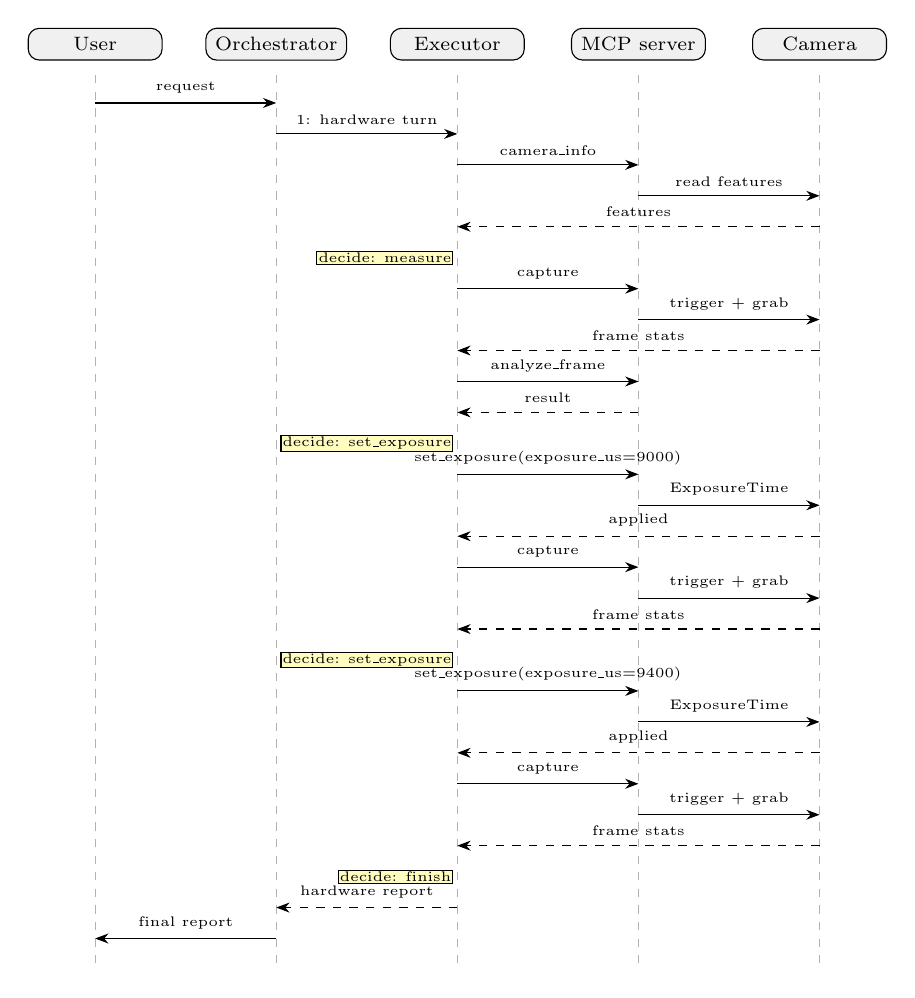
\begin{tikzpicture}[x=1cm,y=-0.393cm,font=\scriptsize,>=Stealth]
\node[draw,fill=gray!12,rounded corners,minimum width=17mm,align=center] at (0.00,-1.4) {User};
\draw[gray!60,dashed] (0.00,-0.4) -- (0.00,28.5);
\node[draw,fill=gray!12,rounded corners,minimum width=17mm,align=center] at (2.30,-1.4) {Orchestrator};
\draw[gray!60,dashed] (2.30,-0.4) -- (2.30,28.5);
\node[draw,fill=gray!12,rounded corners,minimum width=17mm,align=center] at (4.60,-1.4) {Executor};
\draw[gray!60,dashed] (4.60,-0.4) -- (4.60,28.5);
\node[draw,fill=gray!12,rounded corners,minimum width=17mm,align=center] at (6.90,-1.4) {MCP server};
\draw[gray!60,dashed] (6.90,-0.4) -- (6.90,28.5);
\node[draw,fill=gray!12,rounded corners,minimum width=17mm,align=center] at (9.20,-1.4) {Camera};
\draw[gray!60,dashed] (9.20,-0.4) -- (9.20,28.5);
\draw[->] (0.00,0.5) -- node[above,font=\tiny] {request} (2.30,0.5);
\draw[->] (2.30,1.5) -- node[above,font=\tiny] {1: hardware turn} (4.60,1.5);
\draw[->] (4.60,2.5) -- node[above,font=\tiny] {camera\_info} (6.90,2.5);
\draw[->] (6.90,3.5) -- node[above,font=\tiny] {read features} (9.20,3.5);
\draw[->,dashed] (9.20,4.5) -- node[above,font=\tiny] {features} (4.60,4.5);
\node[draw,fill=yellow!25,inner sep=0.6pt,font=\tiny,anchor=east] at (4.55,5.5) {decide: measure};
\draw[->] (4.60,6.5) -- node[above,font=\tiny] {capture} (6.90,6.5);
\draw[->] (6.90,7.5) -- node[above,font=\tiny] {trigger + grab} (9.20,7.5);
\draw[->,dashed] (9.20,8.5) -- node[above,font=\tiny] {frame stats} (4.60,8.5);
\draw[->] (4.60,9.5) -- node[above,font=\tiny] {analyze\_frame} (6.90,9.5);
\draw[->,dashed] (6.90,10.5) -- node[above,font=\tiny] {result} (4.60,10.5);
\node[draw,fill=yellow!25,inner sep=0.6pt,font=\tiny,anchor=east] at (4.55,11.5) {decide: set\_exposure};
\draw[->] (4.60,12.5) -- node[above,font=\tiny] {set\_exposure(exposure\_us=9000)} (6.90,12.5);
\draw[->] (6.90,13.5) -- node[above,font=\tiny] {ExposureTime} (9.20,13.5);
\draw[->,dashed] (9.20,14.5) -- node[above,font=\tiny] {applied} (4.60,14.5);
\draw[->] (4.60,15.5) -- node[above,font=\tiny] {capture} (6.90,15.5);
\draw[->] (6.90,16.5) -- node[above,font=\tiny] {trigger + grab} (9.20,16.5);
\draw[->,dashed] (9.20,17.5) -- node[above,font=\tiny] {frame stats} (4.60,17.5);
\node[draw,fill=yellow!25,inner sep=0.6pt,font=\tiny,anchor=east] at (4.55,18.5) {decide: set\_exposure};
\draw[->] (4.60,19.5) -- node[above,font=\tiny] {set\_exposure(exposure\_us=9400)} (6.90,19.5);
\draw[->] (6.90,20.5) -- node[above,font=\tiny] {ExposureTime} (9.20,20.5);
\draw[->,dashed] (9.20,21.5) -- node[above,font=\tiny] {applied} (4.60,21.5);
\draw[->] (4.60,22.5) -- node[above,font=\tiny] {capture} (6.90,22.5);
\draw[->] (6.90,23.5) -- node[above,font=\tiny] {trigger + grab} (9.20,23.5);
\draw[->,dashed] (9.20,24.5) -- node[above,font=\tiny] {frame stats} (4.60,24.5);
\node[draw,fill=yellow!25,inner sep=0.6pt,font=\tiny,anchor=east] at (4.55,25.5) {decide: finish};
\draw[->,dashed] (4.60,26.5) -- node[above,font=\tiny] {hardware report} (2.30,26.5);
\draw[->] (2.30,27.5) -- node[above,font=\tiny] {final report} (0.00,27.5);
\end{tikzpicture}\end{center}

\clearpage
\subsection*{Use case 4 (real camera): noise model and focusing prediction, the person blocks the light}
\textbf{Request:} \emph{Measure this camera's read noise, conversion gain and full well capacity in electrons. Then use these measured numbers as the camera of the Homework 2 focusing bench and predict the focusing enhancement we can expect with this camera, choosing the bench signal level so that the focus does not saturate it.}\\
Camera: Hikrobot MV-CS028-10UM (real hardware); 5 orchestrator decisions, 12 hardware decisions, 20 MCP tool calls.
\paragraph{Tool calls and what the instrument did.}
{\footnotesize\begin{longtable}{@{}r l p{0.27\linewidth} p{0.52\linewidth}@{}}
\toprule \# & tool & arguments & what the instrument did\\ \midrule \endhead
1 & \texttt{camera\_info} & - & MV-CS028-10UM, 1936x1464, 12-bit; exposure 10000.0 us, gain 0.0 dB\\
2 & \texttt{set\_roi} & x=840, y=604, width=256, height=256 & ROI 256x256 at (840, 604)\\
3 & \texttt{capture} & n\_frames=1, label=roi\_set & 1 frame(s) at 10000 us, 0 dB: mean 63.46, max 74 DN, 0 saturated px\\
4 & \texttt{server\_restart\_restore} & - & server restarted; settings restored \{'roi': [840, 604, 256, 256]\}\\
5 & \texttt{set\_exposure} & exposure\_us=9.0 & exposure set to 9 us\\
6 & \texttt{capture} & n\_frames=16, label=dark\_min & 16 frame(s) at 9 us, 0 dB: mean 62.54, max 70 DN, 0 saturated px; temporal noise 0.9414 DN\\
7 & \texttt{set\_exposure} & exposure\_us=100000.0 & exposure set to 100000 us\\
8 & \texttt{capture} & n\_frames=10, label=dark\_long & 10 frame(s) at 100000 us, 0 dB: mean 63.37, max 153 DN, 0 saturated px; temporal noise 1.0984 DN\\
9 & \texttt{server\_restart\_restore} & - & server restarted; settings restored \{'exposure\_us': 100000.0, 'roi': [840, 604, 256, 256]\}\\
10 & \texttt{capture} & n\_frames=2, label=flat\_test\_100ms & 2 frame(s) at 100000 us, 0 dB: mean 4093.0, max 4093 DN, 0 saturated px; temporal noise 0.0 DN\\
11 & \texttt{set\_exposure} & exposure\_us=20000.0 & exposure set to 20000 us\\
12 & \texttt{capture} & n\_frames=2, label=flat\_test\_20ms & 2 frame(s) at 20000 us, 0 dB: mean 3550.32, max 3667 DN, 0 saturated px; temporal noise 23.8926 DN\\
13 & \texttt{set\_exposure} & exposure\_us=10000.0 & exposure set to 10000 us\\
14 & \texttt{capture} & n\_frames=2, label=flat\_10ms & 2 frame(s) at 10000 us, 0 dB: mean 1819.78, max 1900 DN, 0 saturated px; temporal noise 17.0794 DN\\
15 & \texttt{set\_exposure} & exposure\_us=3000.0 & exposure set to 3000 us\\
16 & \texttt{capture} & n\_frames=8, label=flat\_3ms & 8 frame(s) at 3000 us, 0 dB: mean 587.78, max 632 DN, 0 saturated px; temporal noise 9.4106 DN\\
17 & \texttt{set\_exposure} & exposure\_us=23000.0 & exposure set to 23000 us\\
18 & \texttt{capture} & n\_frames=4, label=flat\_23ms & 4 frame(s) at 23000 us, 0 dB: mean 4071.6, max 4093 DN, 0 saturated px; temporal noise 19.4636 DN\\
19 & \texttt{set\_exposure} & exposure\_us=6000.0 & exposure set to 6000 us\\
20 & \texttt{capture} & n\_frames=6, label=flat\_6ms & 6 frame(s) at 6000 us, 0 dB: mean 1107.92, max 1168 DN, 0 saturated px; temporal noise 13.2053 DN\\
\bottomrule
\end{longtable}}
\paragraph{Sequence diagram.} Solid arrows: messages and commands; dashed: replies and measurements; boxes: the executor's decisions (model calls). Numbers are the orchestrator's decision index.
\begin{center}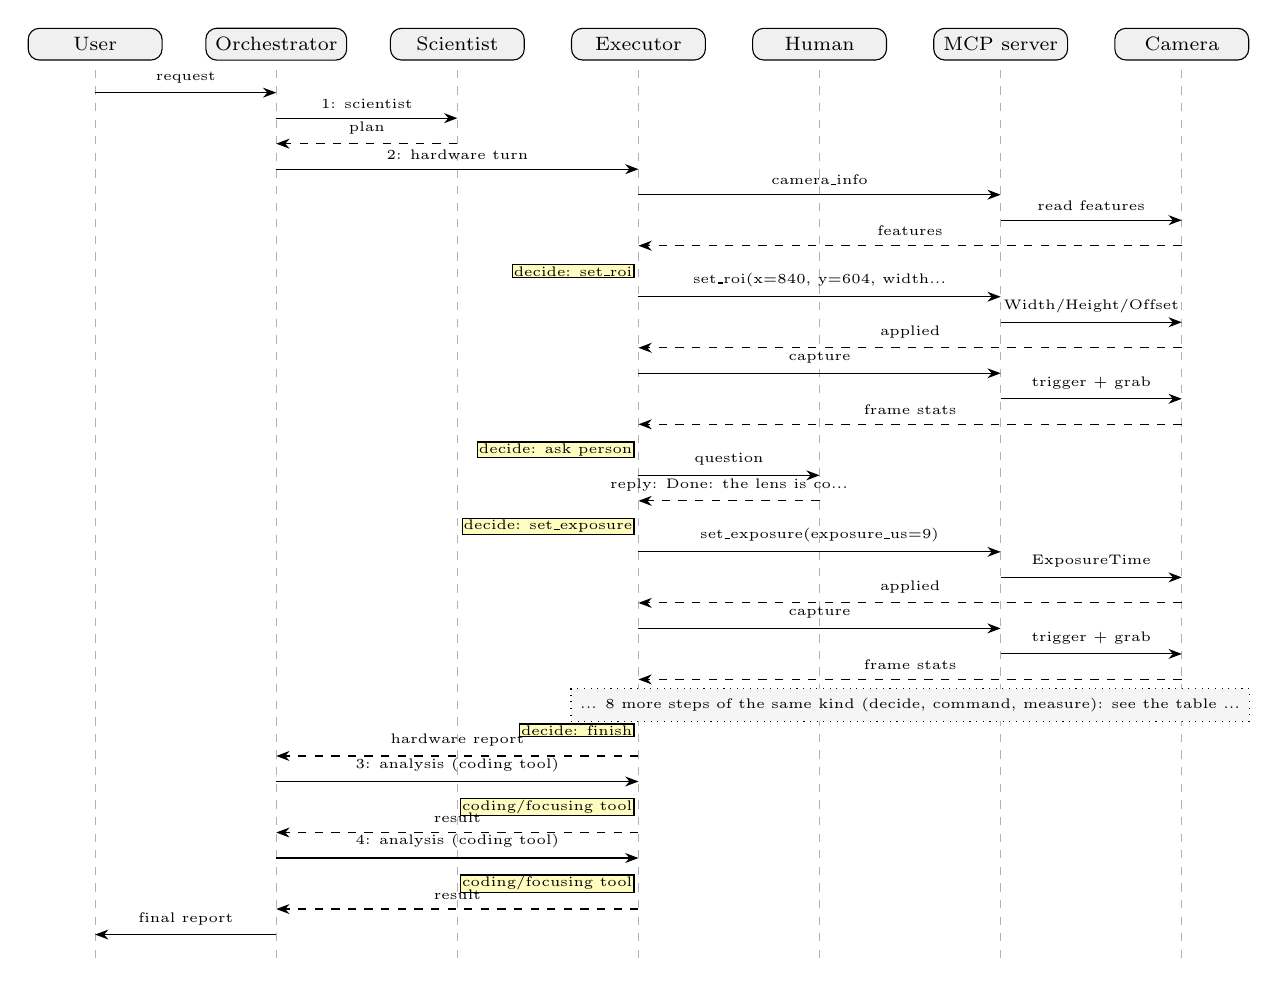
\begin{tikzpicture}[x=1cm,y=-0.324cm,font=\scriptsize,>=Stealth]
\node[draw,fill=gray!12,rounded corners,minimum width=17mm,align=center] at (0.00,-1.4) {User};
\draw[gray!60,dashed] (0.00,-0.4) -- (0.00,34.5);
\node[draw,fill=gray!12,rounded corners,minimum width=17mm,align=center] at (2.30,-1.4) {Orchestrator};
\draw[gray!60,dashed] (2.30,-0.4) -- (2.30,34.5);
\node[draw,fill=gray!12,rounded corners,minimum width=17mm,align=center] at (4.60,-1.4) {Scientist};
\draw[gray!60,dashed] (4.60,-0.4) -- (4.60,34.5);
\node[draw,fill=gray!12,rounded corners,minimum width=17mm,align=center] at (6.90,-1.4) {Executor};
\draw[gray!60,dashed] (6.90,-0.4) -- (6.90,34.5);
\node[draw,fill=gray!12,rounded corners,minimum width=17mm,align=center] at (9.20,-1.4) {Human};
\draw[gray!60,dashed] (9.20,-0.4) -- (9.20,34.5);
\node[draw,fill=gray!12,rounded corners,minimum width=17mm,align=center] at (11.50,-1.4) {MCP server};
\draw[gray!60,dashed] (11.50,-0.4) -- (11.50,34.5);
\node[draw,fill=gray!12,rounded corners,minimum width=17mm,align=center] at (13.80,-1.4) {Camera};
\draw[gray!60,dashed] (13.80,-0.4) -- (13.80,34.5);
\draw[->] (0.00,0.5) -- node[above,font=\tiny] {request} (2.30,0.5);
\draw[->] (2.30,1.5) -- node[above,font=\tiny] {1: scientist} (4.60,1.5);
\draw[->,dashed] (4.60,2.5) -- node[above,font=\tiny] {plan} (2.30,2.5);
\draw[->] (2.30,3.5) -- node[above,font=\tiny] {2: hardware turn} (6.90,3.5);
\draw[->] (6.90,4.5) -- node[above,font=\tiny] {camera\_info} (11.50,4.5);
\draw[->] (11.50,5.5) -- node[above,font=\tiny] {read features} (13.80,5.5);
\draw[->,dashed] (13.80,6.5) -- node[above,font=\tiny] {features} (6.90,6.5);
\node[draw,fill=yellow!25,inner sep=0.6pt,font=\tiny,anchor=east] at (6.85,7.5) {decide: set\_roi};
\draw[->] (6.90,8.5) -- node[above,font=\tiny] {set\_roi(x=840, y=604, width...} (11.50,8.5);
\draw[->] (11.50,9.5) -- node[above,font=\tiny] {Width/Height/Offset} (13.80,9.5);
\draw[->,dashed] (13.80,10.5) -- node[above,font=\tiny] {applied} (6.90,10.5);
\draw[->] (6.90,11.5) -- node[above,font=\tiny] {capture} (11.50,11.5);
\draw[->] (11.50,12.5) -- node[above,font=\tiny] {trigger + grab} (13.80,12.5);
\draw[->,dashed] (13.80,13.5) -- node[above,font=\tiny] {frame stats} (6.90,13.5);
\node[draw,fill=yellow!25,inner sep=0.6pt,font=\tiny,anchor=east] at (6.85,14.5) {decide: ask person};
\draw[->] (6.90,15.5) -- node[above,font=\tiny] {question} (9.20,15.5);
\draw[->,dashed] (9.20,16.5) -- node[above,font=\tiny] {reply: Done: the lens is co...} (6.90,16.5);
\node[draw,fill=yellow!25,inner sep=0.6pt,font=\tiny,anchor=east] at (6.85,17.5) {decide: set\_exposure};
\draw[->] (6.90,18.5) -- node[above,font=\tiny] {set\_exposure(exposure\_us=9)} (11.50,18.5);
\draw[->] (11.50,19.5) -- node[above,font=\tiny] {ExposureTime} (13.80,19.5);
\draw[->,dashed] (13.80,20.5) -- node[above,font=\tiny] {applied} (6.90,20.5);
\draw[->] (6.90,21.5) -- node[above,font=\tiny] {capture} (11.50,21.5);
\draw[->] (11.50,22.5) -- node[above,font=\tiny] {trigger + grab} (13.80,22.5);
\draw[->,dashed] (13.80,23.5) -- node[above,font=\tiny] {frame stats} (6.90,23.5);
\node[draw,dotted,fill=gray!8,font=\tiny,minimum width=7.30cm] at (10.35,24.5) {... 8 more steps of the same kind (decide, command, measure): see the table ...};
\node[draw,fill=yellow!25,inner sep=0.6pt,font=\tiny,anchor=east] at (6.85,25.5) {decide: finish};
\draw[->,dashed] (6.90,26.5) -- node[above,font=\tiny] {hardware report} (2.30,26.5);
\draw[->] (2.30,27.5) -- node[above,font=\tiny] {3: analysis (coding tool)} (6.90,27.5);
\node[draw,fill=yellow!25,inner sep=0.6pt,font=\tiny,anchor=east] at (6.85,28.5) {coding/focusing tool};
\draw[->,dashed] (6.90,29.5) -- node[above,font=\tiny] {result} (2.30,29.5);
\draw[->] (2.30,30.5) -- node[above,font=\tiny] {4: analysis (coding tool)} (6.90,30.5);
\node[draw,fill=yellow!25,inner sep=0.6pt,font=\tiny,anchor=east] at (6.85,31.5) {coding/focusing tool};
\draw[->,dashed] (6.90,32.5) -- node[above,font=\tiny] {result} (2.30,32.5);
\draw[->] (2.30,33.5) -- node[above,font=\tiny] {final report} (0.00,33.5);
\end{tikzpicture}\end{center}

\clearpage
\subsection*{Use case 6 (real camera): human stops (second video)}
\textbf{Request:} \emph{Set the gain to 12 dB and choose the exposure so that the wall is at about half of the camera's range, then report the exposure and the temporal noise.}\\
Camera: Hikrobot MV-CS028-10UM (real hardware); 3 orchestrator decisions, 3 hardware decisions, 6 MCP tool calls.
\paragraph{Tool calls and what the instrument did.}
{\footnotesize\begin{longtable}{@{}r l p{0.27\linewidth} p{0.52\linewidth}@{}}
\toprule \# & tool & arguments & what the instrument did\\ \midrule \endhead
1 & \texttt{camera\_info} & - & MV-CS028-10UM, 1936x1464, 12-bit; exposure 3250.0 us, gain 11.991 dB\\
2 & \texttt{set\_gain} & gain\_db=12.0 & gain set to 11.991 dB\\
3 & \texttt{capture} & n\_frames=5, label=iter\_1 & 5 frame(s) at 3250 us, 11.991 dB: mean 1626.1, max 1765 DN, 0 saturated px; temporal noise 32.2099 DN\\
4 & \texttt{analyze\_frame} & frame\_file=cap001\_iter\_1.npy, black\_level\_dn=0.0 & speckle contrast 0.0204, grain 0.999 x 1.034 px; beam centroid (127.5, 127.6) px\\
5 & \texttt{set\_exposure} & exposure\_us=4090.0 & exposure set to 4090 us\\
6 & \texttt{capture} & n\_frames=5, label=iter\_2 & 5 frame(s) at 4090 us, 11.991 dB: mean 2030.38, max 2201 DN, 0 saturated px; temporal noise 35.9004 DN\\
\bottomrule
\end{longtable}}
\paragraph{Sequence diagram.} Solid arrows: messages and commands; dashed: replies and measurements; boxes: the executor's decisions (model calls). Numbers are the orchestrator's decision index.
\begin{center}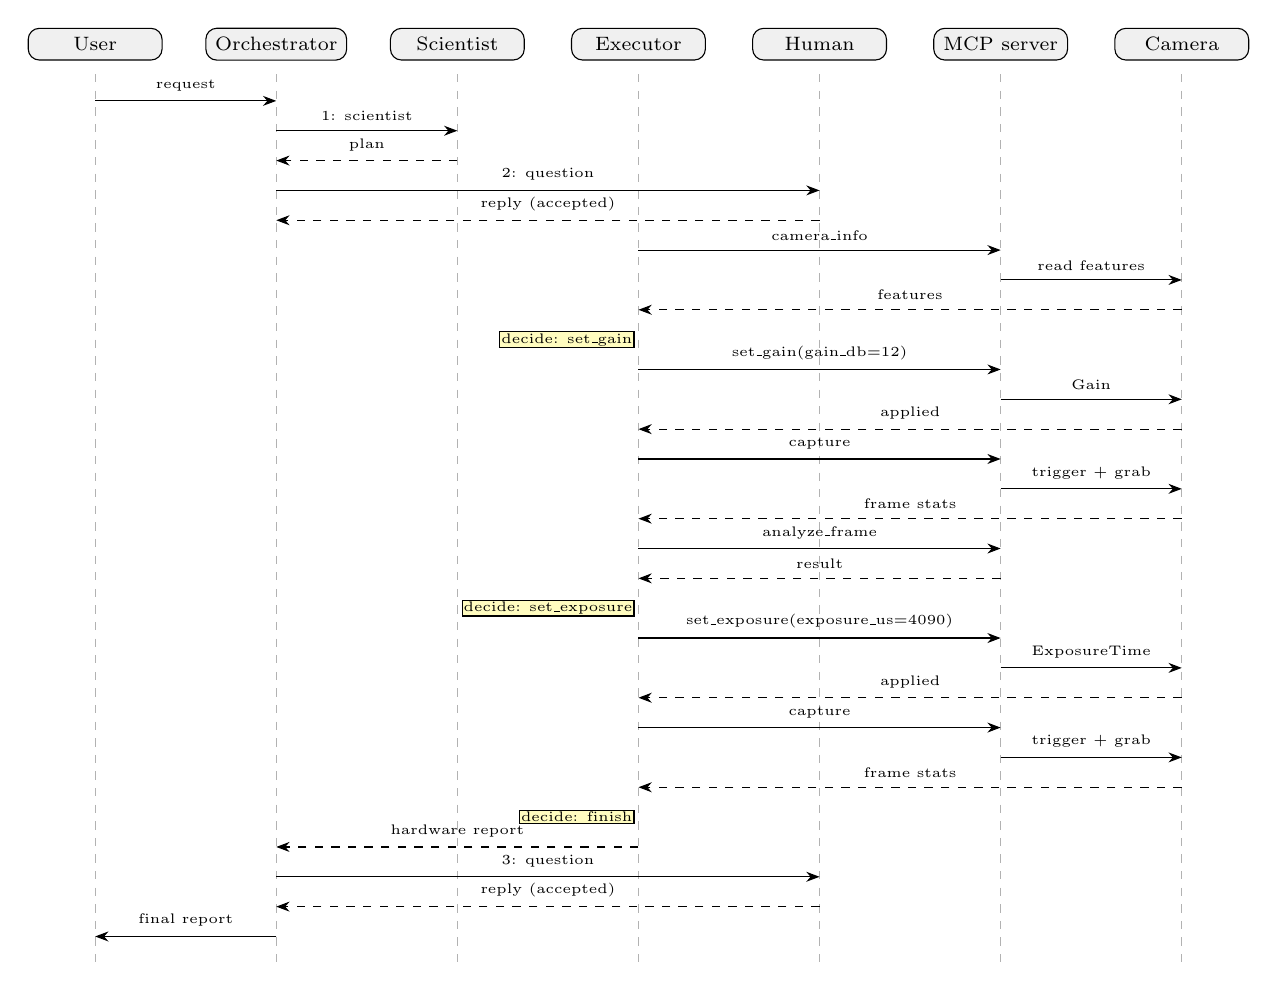
\begin{tikzpicture}[x=1cm,y=-0.379cm,font=\scriptsize,>=Stealth]
\node[draw,fill=gray!12,rounded corners,minimum width=17mm,align=center] at (0.00,-1.4) {User};
\draw[gray!60,dashed] (0.00,-0.4) -- (0.00,29.5);
\node[draw,fill=gray!12,rounded corners,minimum width=17mm,align=center] at (2.30,-1.4) {Orchestrator};
\draw[gray!60,dashed] (2.30,-0.4) -- (2.30,29.5);
\node[draw,fill=gray!12,rounded corners,minimum width=17mm,align=center] at (4.60,-1.4) {Scientist};
\draw[gray!60,dashed] (4.60,-0.4) -- (4.60,29.5);
\node[draw,fill=gray!12,rounded corners,minimum width=17mm,align=center] at (6.90,-1.4) {Executor};
\draw[gray!60,dashed] (6.90,-0.4) -- (6.90,29.5);
\node[draw,fill=gray!12,rounded corners,minimum width=17mm,align=center] at (9.20,-1.4) {Human};
\draw[gray!60,dashed] (9.20,-0.4) -- (9.20,29.5);
\node[draw,fill=gray!12,rounded corners,minimum width=17mm,align=center] at (11.50,-1.4) {MCP server};
\draw[gray!60,dashed] (11.50,-0.4) -- (11.50,29.5);
\node[draw,fill=gray!12,rounded corners,minimum width=17mm,align=center] at (13.80,-1.4) {Camera};
\draw[gray!60,dashed] (13.80,-0.4) -- (13.80,29.5);
\draw[->] (0.00,0.5) -- node[above,font=\tiny] {request} (2.30,0.5);
\draw[->] (2.30,1.5) -- node[above,font=\tiny] {1: scientist} (4.60,1.5);
\draw[->,dashed] (4.60,2.5) -- node[above,font=\tiny] {plan} (2.30,2.5);
\draw[->] (2.30,3.5) -- node[above,font=\tiny] {2: question} (9.20,3.5);
\draw[->,dashed] (9.20,4.5) -- node[above,font=\tiny] {reply (accepted)} (2.30,4.5);
\draw[->] (6.90,5.5) -- node[above,font=\tiny] {camera\_info} (11.50,5.5);
\draw[->] (11.50,6.5) -- node[above,font=\tiny] {read features} (13.80,6.5);
\draw[->,dashed] (13.80,7.5) -- node[above,font=\tiny] {features} (6.90,7.5);
\node[draw,fill=yellow!25,inner sep=0.6pt,font=\tiny,anchor=east] at (6.85,8.5) {decide: set\_gain};
\draw[->] (6.90,9.5) -- node[above,font=\tiny] {set\_gain(gain\_db=12)} (11.50,9.5);
\draw[->] (11.50,10.5) -- node[above,font=\tiny] {Gain} (13.80,10.5);
\draw[->,dashed] (13.80,11.5) -- node[above,font=\tiny] {applied} (6.90,11.5);
\draw[->] (6.90,12.5) -- node[above,font=\tiny] {capture} (11.50,12.5);
\draw[->] (11.50,13.5) -- node[above,font=\tiny] {trigger + grab} (13.80,13.5);
\draw[->,dashed] (13.80,14.5) -- node[above,font=\tiny] {frame stats} (6.90,14.5);
\draw[->] (6.90,15.5) -- node[above,font=\tiny] {analyze\_frame} (11.50,15.5);
\draw[->,dashed] (11.50,16.5) -- node[above,font=\tiny] {result} (6.90,16.5);
\node[draw,fill=yellow!25,inner sep=0.6pt,font=\tiny,anchor=east] at (6.85,17.5) {decide: set\_exposure};
\draw[->] (6.90,18.5) -- node[above,font=\tiny] {set\_exposure(exposure\_us=4090)} (11.50,18.5);
\draw[->] (11.50,19.5) -- node[above,font=\tiny] {ExposureTime} (13.80,19.5);
\draw[->,dashed] (13.80,20.5) -- node[above,font=\tiny] {applied} (6.90,20.5);
\draw[->] (6.90,21.5) -- node[above,font=\tiny] {capture} (11.50,21.5);
\draw[->] (11.50,22.5) -- node[above,font=\tiny] {trigger + grab} (13.80,22.5);
\draw[->,dashed] (13.80,23.5) -- node[above,font=\tiny] {frame stats} (6.90,23.5);
\node[draw,fill=yellow!25,inner sep=0.6pt,font=\tiny,anchor=east] at (6.85,24.5) {decide: finish};
\draw[->,dashed] (6.90,25.5) -- node[above,font=\tiny] {hardware report} (2.30,25.5);
\draw[->] (2.30,26.5) -- node[above,font=\tiny] {3: question} (9.20,26.5);
\draw[->,dashed] (9.20,27.5) -- node[above,font=\tiny] {reply (accepted)} (2.30,27.5);
\draw[->] (2.30,28.5) -- node[above,font=\tiny] {final report} (0.00,28.5);
\end{tikzpicture}\end{center}

\clearpage
\subsection*{Use case 2 (real camera): flicker-free exposure}
\textbf{Request:} \emph{The camera looks at a white surface under the lab's room lights, which may flicker. Find an exposure at which the frame-to-frame brightness is stable, with the image well exposed but not saturated, and report how strong the flicker is at a short exposure and at the exposure you chose.}\\
Camera: Hikrobot MV-CS028-10UM (real hardware); 3 orchestrator decisions, 13 hardware decisions, 23 MCP tool calls.
\\{\small\textbf{Tool calls and what the instrument did:} (1)~\texttt{camera\_info} $\to$ MV-CS028-10UM, 1936x1464, 12-bit; exposure 9400.0 us, gain 0.0 dB; (2)~\texttt{set\_roi} x=768, y=532, width=400, height=400 $\to$ ROI 400x400 at (768, 532); (3)~\texttt{capture} n\_frames=1 $\to$ 1 frame(s) at 9400 us, 0 dB: mean 2313.58, max 2409 DN, 0 saturated px; (4)~\texttt{set\_exposure} exposure\_us=1000.0 $\to$ exposure set to 1000 us; (5)~\texttt{capture} n\_frames=16, label=short\_1000 $\to$ 16 frame(s) at 1000 us, 0 dB: mean 301.09, max 331 DN, 0 saturated ...; (6)~\texttt{set\_exposure} exposure\_us=2000.0 $\to$ exposure set to 2000 us; (7)~\texttt{capture} n\_frames=16, label=short\_2000 $\to$ 16 frame(s) at 2000 us, 0 dB: mean 540.24, max 583 DN, 0 saturated ...; (8)~\texttt{set\_exposure} exposure\_us=5000.0 $\to$ exposure set to 5000 us; (9)~\texttt{capture} n\_frames=16, label=scan\_5000 $\to$ 16 frame(s) at 5000 us, 0 dB: mean 1251.61, max 1317 DN, 0 saturate...; (10)~\texttt{set\_exposure} exposure\_us=8333.0 $\to$ exposure set to 8333 us; (11)~\texttt{capture} n\_frames=16, label=scan\_8333 $\to$ 16 frame(s) at 8333 us, 0 dB: mean 2041.56, max 2130 DN, 0 saturate...; (12)~\texttt{set\_exposure} exposure\_us=10000.0 $\to$ exposure set to 10000 us; (13)~\texttt{capture} n\_frames=16, label=scan\_10000 $\to$ 16 frame(s) at 10000 us, 0 dB: mean 2436.85, max 2534 DN, 0 saturat...; (14)~\texttt{set\_exposure} exposure\_us=12000.0 $\to$ exposure set to 12000 us; (15)~\texttt{capture} n\_frames=16, label=scan\_12000 $\to$ 16 frame(s) at 12000 us, 0 dB: mean 2902.14, max 3015 DN, 0 saturat...; (16)~\texttt{set\_exposure} exposure\_us=16667.0 $\to$ exposure set to 16667 us; (17)~\texttt{capture} n\_frames=16, label=scan\_16667 $\to$ 16 frame(s) at 16667 us, 0 dB: mean 3994.7, max 4093 DN, 0 saturate...; (18)~\texttt{set\_exposure} exposure\_us=1000.0 $\to$ exposure set to 1000 us; (19)~\texttt{capture} n\_frames=1, label=short\_1000\_series $\to$ 1 frame(s) at 1000 us, 0 dB: mean 297.33, max 330 DN, 0 saturated px; (20)~\texttt{capture\_series} n\_frames=16, interval\_s=0.137, label=... $\to$ 16 frames over 2.06 s: mean 296.892 DN, rel. std 0.1411\%, drift -0....; (21)~\texttt{set\_exposure} exposure\_us=10000.0 $\to$ exposure set to 10000 us; (22)~\texttt{capture} n\_frames=1, label=series\_10000\_pre $\to$ 1 frame(s) at 10000 us, 0 dB: mean 2398.35, max 2497 DN, 0 saturate...; (23)~\texttt{capture\_series} n\_frames=16, interval\_s=0.137, label=... $\to$ 16 frames over 2.069 s: mean 2390.202 DN, rel. std 0.0494\%, drift 0....}
\\\textbf{Verified result:} 10000 us, 0 dB: max 2497 DN, 0 saturated px.
\par\smallskip\textbf{Sequence diagram} (as above; long hardware turns shortened).
\begin{center}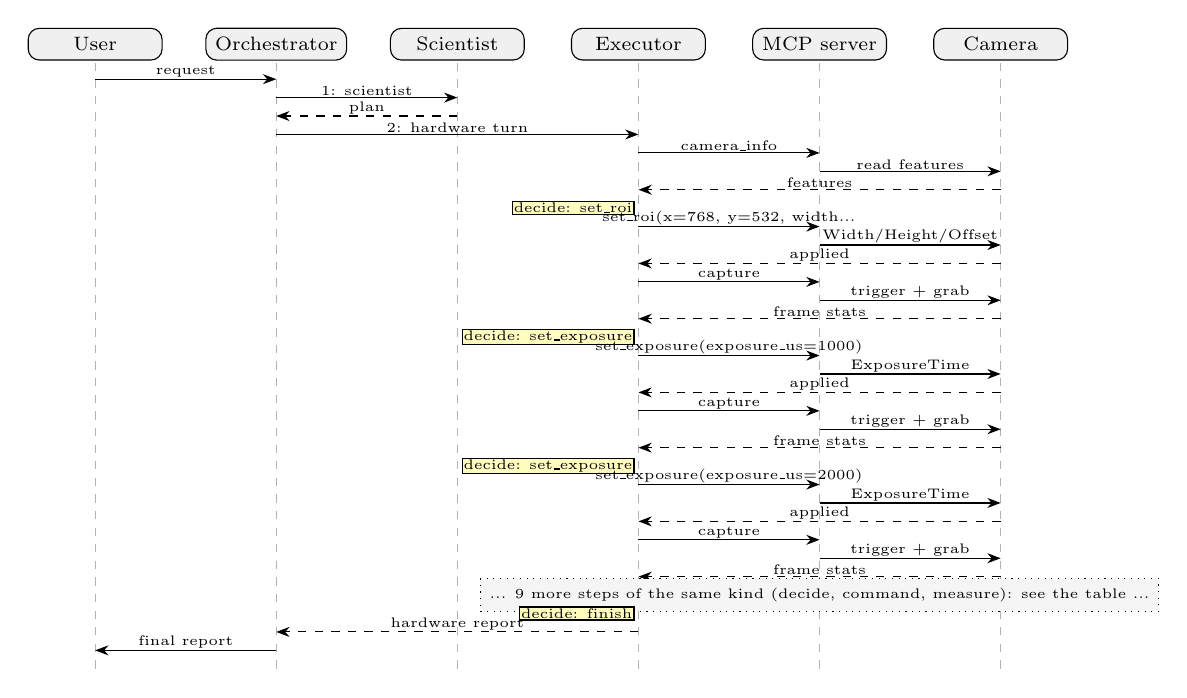
\begin{tikzpicture}[x=1cm,y=-0.234cm,font=\scriptsize,>=Stealth]
\node[draw,fill=gray!12,rounded corners,minimum width=17mm,align=center] at (0.00,-1.4) {User};
\draw[gray!60,dashed] (0.00,-0.4) -- (0.00,32.5);
\node[draw,fill=gray!12,rounded corners,minimum width=17mm,align=center] at (2.30,-1.4) {Orchestrator};
\draw[gray!60,dashed] (2.30,-0.4) -- (2.30,32.5);
\node[draw,fill=gray!12,rounded corners,minimum width=17mm,align=center] at (4.60,-1.4) {Scientist};
\draw[gray!60,dashed] (4.60,-0.4) -- (4.60,32.5);
\node[draw,fill=gray!12,rounded corners,minimum width=17mm,align=center] at (6.90,-1.4) {Executor};
\draw[gray!60,dashed] (6.90,-0.4) -- (6.90,32.5);
\node[draw,fill=gray!12,rounded corners,minimum width=17mm,align=center] at (9.20,-1.4) {MCP server};
\draw[gray!60,dashed] (9.20,-0.4) -- (9.20,32.5);
\node[draw,fill=gray!12,rounded corners,minimum width=17mm,align=center] at (11.50,-1.4) {Camera};
\draw[gray!60,dashed] (11.50,-0.4) -- (11.50,32.5);
\draw[->] (0.00,0.5) -- node[above,inner sep=0.5pt,font=\tiny] {request} (2.30,0.5);
\draw[->] (2.30,1.5) -- node[above,inner sep=0.5pt,font=\tiny] {1: scientist} (4.60,1.5);
\draw[->,dashed] (4.60,2.5) -- node[above,inner sep=0.5pt,font=\tiny] {plan} (2.30,2.5);
\draw[->] (2.30,3.5) -- node[above,inner sep=0.5pt,font=\tiny] {2: hardware turn} (6.90,3.5);
\draw[->] (6.90,4.5) -- node[above,inner sep=0.5pt,font=\tiny] {camera\_info} (9.20,4.5);
\draw[->] (9.20,5.5) -- node[above,inner sep=0.5pt,font=\tiny] {read features} (11.50,5.5);
\draw[->,dashed] (11.50,6.5) -- node[above,inner sep=0.5pt,font=\tiny] {features} (6.90,6.5);
\node[draw,fill=yellow!25,inner sep=0.6pt,font=\tiny,anchor=east] at (6.85,7.5) {decide: set\_roi};
\draw[->] (6.90,8.5) -- node[above,inner sep=0.5pt,font=\tiny] {set\_roi(x=768, y=532, width...} (9.20,8.5);
\draw[->] (9.20,9.5) -- node[above,inner sep=0.5pt,font=\tiny] {Width/Height/Offset} (11.50,9.5);
\draw[->,dashed] (11.50,10.5) -- node[above,inner sep=0.5pt,font=\tiny] {applied} (6.90,10.5);
\draw[->] (6.90,11.5) -- node[above,inner sep=0.5pt,font=\tiny] {capture} (9.20,11.5);
\draw[->] (9.20,12.5) -- node[above,inner sep=0.5pt,font=\tiny] {trigger + grab} (11.50,12.5);
\draw[->,dashed] (11.50,13.5) -- node[above,inner sep=0.5pt,font=\tiny] {frame stats} (6.90,13.5);
\node[draw,fill=yellow!25,inner sep=0.6pt,font=\tiny,anchor=east] at (6.85,14.5) {decide: set\_exposure};
\draw[->] (6.90,15.5) -- node[above,inner sep=0.5pt,font=\tiny] {set\_exposure(exposure\_us=1000)} (9.20,15.5);
\draw[->] (9.20,16.5) -- node[above,inner sep=0.5pt,font=\tiny] {ExposureTime} (11.50,16.5);
\draw[->,dashed] (11.50,17.5) -- node[above,inner sep=0.5pt,font=\tiny] {applied} (6.90,17.5);
\draw[->] (6.90,18.5) -- node[above,inner sep=0.5pt,font=\tiny] {capture} (9.20,18.5);
\draw[->] (9.20,19.5) -- node[above,inner sep=0.5pt,font=\tiny] {trigger + grab} (11.50,19.5);
\draw[->,dashed] (11.50,20.5) -- node[above,inner sep=0.5pt,font=\tiny] {frame stats} (6.90,20.5);
\node[draw,fill=yellow!25,inner sep=0.6pt,font=\tiny,anchor=east] at (6.85,21.5) {decide: set\_exposure};
\draw[->] (6.90,22.5) -- node[above,inner sep=0.5pt,font=\tiny] {set\_exposure(exposure\_us=2000)} (9.20,22.5);
\draw[->] (9.20,23.5) -- node[above,inner sep=0.5pt,font=\tiny] {ExposureTime} (11.50,23.5);
\draw[->,dashed] (11.50,24.5) -- node[above,inner sep=0.5pt,font=\tiny] {applied} (6.90,24.5);
\draw[->] (6.90,25.5) -- node[above,inner sep=0.5pt,font=\tiny] {capture} (9.20,25.5);
\draw[->] (9.20,26.5) -- node[above,inner sep=0.5pt,font=\tiny] {trigger + grab} (11.50,26.5);
\draw[->,dashed] (11.50,27.5) -- node[above,inner sep=0.5pt,font=\tiny] {frame stats} (6.90,27.5);
\node[draw,dotted,fill=gray!8,font=\tiny,minimum width=5.00cm] at (9.20,28.5) {... 9 more steps of the same kind (decide, command, measure): see the table ...};
\node[draw,fill=yellow!25,inner sep=0.6pt,font=\tiny,anchor=east] at (6.85,29.5) {decide: finish};
\draw[->,dashed] (6.90,30.5) -- node[above,inner sep=0.5pt,font=\tiny] {hardware report} (2.30,30.5);
\draw[->] (2.30,31.5) -- node[above,inner sep=0.5pt,font=\tiny] {final report} (0.00,31.5);
\end{tikzpicture}\end{center}

\subsection*{Use case 3 (real camera): stability, the person blocks the light}
\textbf{Request:} \emph{At an exposure free of the light flicker, measure how stable the brightness is over two minutes and report the drift.}\\
Camera: Hikrobot MV-CS028-10UM (real hardware); 4 orchestrator decisions, 8 hardware decisions, 11 MCP tool calls.
\\{\small\textbf{Tool calls and what the instrument did:} (1)~\texttt{camera\_info} $\to$ MV-CS028-10UM, 1936x1464, 12-bit; exposure 10000.0 us, gain 0.0 dB; (2)~\texttt{capture} n\_frames=4, label=baseline\_10ms $\to$ 4 frame(s) at 10000 us, 0 dB: mean 2274.07, max 2368 DN, 0 saturate...; (3)~\texttt{set\_exposure} exposure\_us=15000.0 $\to$ exposure set to 15000 us; (4)~\texttt{capture} n\_frames=16, label=scan\_15ms $\to$ 16 frame(s) at 15000 us, 0 dB: mean 3362.9, max 3497 DN, 0 saturate...; (5)~\texttt{set\_exposure} exposure\_us=5000.0 $\to$ exposure set to 5000 us; (6)~\texttt{capture} n\_frames=16, label=scan\_5ms $\to$ 16 frame(s) at 5000 us, 0 dB: mean 1156.75, max 1221 DN, 0 saturate...; (7)~\texttt{set\_exposure} exposure\_us=10000.0 $\to$ exposure set to 10000 us; (8)~\texttt{capture} n\_frames=16, label=scan\_10ms $\to$ 16 frame(s) at 10000 us, 0 dB: mean 2244.14, max 2359 DN, 0 saturat...; (9)~\texttt{capture\_series} n\_frames=121, interval\_s=1.0, label=d... $\to$ 121 frames over 120.014 s: mean 2153.35 DN, rel. std 1.942\%, drift ...; (10)~\texttt{server\_restart\_restore} $\to$ server restarted; settings restored \{'exposure\_us': 10000.0\}; (11)~\texttt{capture} n\_frames=16, label=dark\_after $\to$ 16 frame(s) at 10000 us, 0 dB: mean 63.4, max 75 DN, 0 saturated px....}
\\\textbf{Verified result:} script drift\_analysis.py: SLOPE\_PCT\_PER\_MIN=-3.43, TOTAL\_CHANGE\_PCT=-6.859, FLICKER\_NFRAMES\_5ms=16, FLICKER\_MEAN\_DN\_5ms=1157.
\par\smallskip\textbf{Sequence diagram} (as above; long hardware turns shortened).
\begin{center}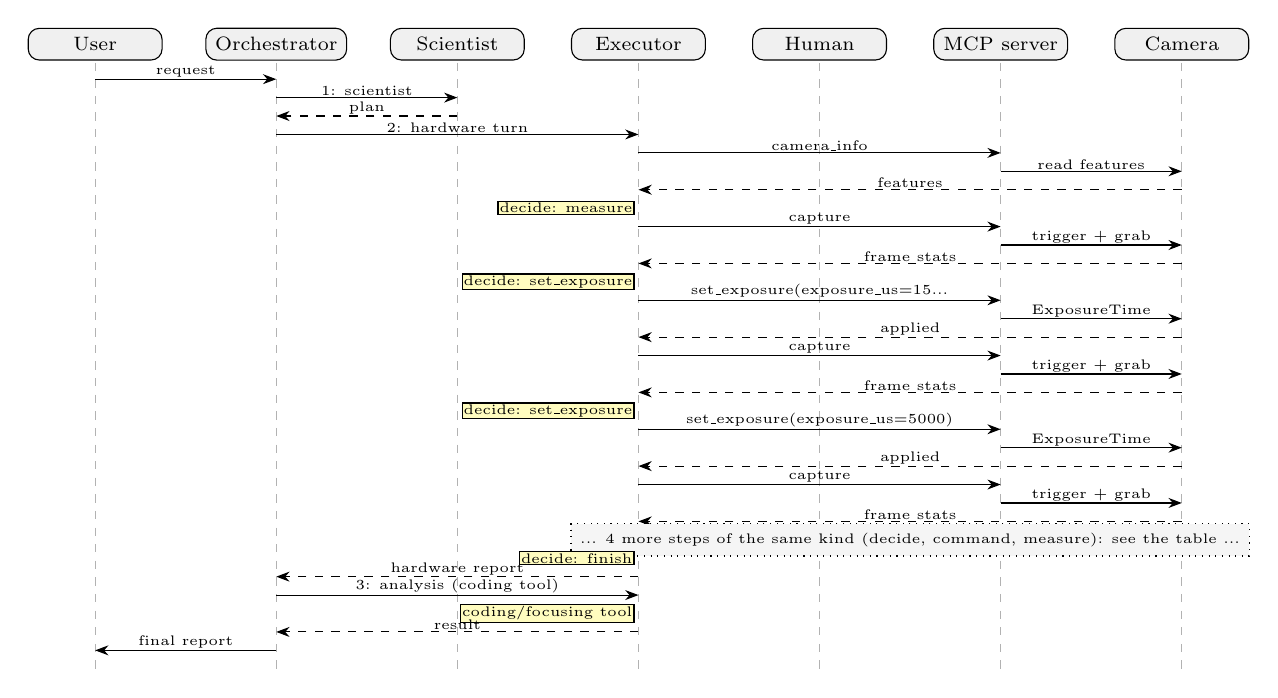
\begin{tikzpicture}[x=1cm,y=-0.234cm,font=\scriptsize,>=Stealth]
\node[draw,fill=gray!12,rounded corners,minimum width=17mm,align=center] at (0.00,-1.4) {User};
\draw[gray!60,dashed] (0.00,-0.4) -- (0.00,32.5);
\node[draw,fill=gray!12,rounded corners,minimum width=17mm,align=center] at (2.30,-1.4) {Orchestrator};
\draw[gray!60,dashed] (2.30,-0.4) -- (2.30,32.5);
\node[draw,fill=gray!12,rounded corners,minimum width=17mm,align=center] at (4.60,-1.4) {Scientist};
\draw[gray!60,dashed] (4.60,-0.4) -- (4.60,32.5);
\node[draw,fill=gray!12,rounded corners,minimum width=17mm,align=center] at (6.90,-1.4) {Executor};
\draw[gray!60,dashed] (6.90,-0.4) -- (6.90,32.5);
\node[draw,fill=gray!12,rounded corners,minimum width=17mm,align=center] at (9.20,-1.4) {Human};
\draw[gray!60,dashed] (9.20,-0.4) -- (9.20,32.5);
\node[draw,fill=gray!12,rounded corners,minimum width=17mm,align=center] at (11.50,-1.4) {MCP server};
\draw[gray!60,dashed] (11.50,-0.4) -- (11.50,32.5);
\node[draw,fill=gray!12,rounded corners,minimum width=17mm,align=center] at (13.80,-1.4) {Camera};
\draw[gray!60,dashed] (13.80,-0.4) -- (13.80,32.5);
\draw[->] (0.00,0.5) -- node[above,inner sep=0.5pt,font=\tiny] {request} (2.30,0.5);
\draw[->] (2.30,1.5) -- node[above,inner sep=0.5pt,font=\tiny] {1: scientist} (4.60,1.5);
\draw[->,dashed] (4.60,2.5) -- node[above,inner sep=0.5pt,font=\tiny] {plan} (2.30,2.5);
\draw[->] (2.30,3.5) -- node[above,inner sep=0.5pt,font=\tiny] {2: hardware turn} (6.90,3.5);
\draw[->] (6.90,4.5) -- node[above,inner sep=0.5pt,font=\tiny] {camera\_info} (11.50,4.5);
\draw[->] (11.50,5.5) -- node[above,inner sep=0.5pt,font=\tiny] {read features} (13.80,5.5);
\draw[->,dashed] (13.80,6.5) -- node[above,inner sep=0.5pt,font=\tiny] {features} (6.90,6.5);
\node[draw,fill=yellow!25,inner sep=0.6pt,font=\tiny,anchor=east] at (6.85,7.5) {decide: measure};
\draw[->] (6.90,8.5) -- node[above,inner sep=0.5pt,font=\tiny] {capture} (11.50,8.5);
\draw[->] (11.50,9.5) -- node[above,inner sep=0.5pt,font=\tiny] {trigger + grab} (13.80,9.5);
\draw[->,dashed] (13.80,10.5) -- node[above,inner sep=0.5pt,font=\tiny] {frame stats} (6.90,10.5);
\node[draw,fill=yellow!25,inner sep=0.6pt,font=\tiny,anchor=east] at (6.85,11.5) {decide: set\_exposure};
\draw[->] (6.90,12.5) -- node[above,inner sep=0.5pt,font=\tiny] {set\_exposure(exposure\_us=15...} (11.50,12.5);
\draw[->] (11.50,13.5) -- node[above,inner sep=0.5pt,font=\tiny] {ExposureTime} (13.80,13.5);
\draw[->,dashed] (13.80,14.5) -- node[above,inner sep=0.5pt,font=\tiny] {applied} (6.90,14.5);
\draw[->] (6.90,15.5) -- node[above,inner sep=0.5pt,font=\tiny] {capture} (11.50,15.5);
\draw[->] (11.50,16.5) -- node[above,inner sep=0.5pt,font=\tiny] {trigger + grab} (13.80,16.5);
\draw[->,dashed] (13.80,17.5) -- node[above,inner sep=0.5pt,font=\tiny] {frame stats} (6.90,17.5);
\node[draw,fill=yellow!25,inner sep=0.6pt,font=\tiny,anchor=east] at (6.85,18.5) {decide: set\_exposure};
\draw[->] (6.90,19.5) -- node[above,inner sep=0.5pt,font=\tiny] {set\_exposure(exposure\_us=5000)} (11.50,19.5);
\draw[->] (11.50,20.5) -- node[above,inner sep=0.5pt,font=\tiny] {ExposureTime} (13.80,20.5);
\draw[->,dashed] (13.80,21.5) -- node[above,inner sep=0.5pt,font=\tiny] {applied} (6.90,21.5);
\draw[->] (6.90,22.5) -- node[above,inner sep=0.5pt,font=\tiny] {capture} (11.50,22.5);
\draw[->] (11.50,23.5) -- node[above,inner sep=0.5pt,font=\tiny] {trigger + grab} (13.80,23.5);
\draw[->,dashed] (13.80,24.5) -- node[above,inner sep=0.5pt,font=\tiny] {frame stats} (6.90,24.5);
\node[draw,dotted,fill=gray!8,font=\tiny,minimum width=7.30cm] at (10.35,25.5) {... 4 more steps of the same kind (decide, command, measure): see the table ...};
\node[draw,fill=yellow!25,inner sep=0.6pt,font=\tiny,anchor=east] at (6.85,26.5) {decide: finish};
\draw[->,dashed] (6.90,27.5) -- node[above,inner sep=0.5pt,font=\tiny] {hardware report} (2.30,27.5);
\draw[->] (2.30,28.5) -- node[above,inner sep=0.5pt,font=\tiny] {3: analysis (coding tool)} (6.90,28.5);
\node[draw,fill=yellow!25,inner sep=0.6pt,font=\tiny,anchor=east] at (6.85,29.5) {coding/focusing tool};
\draw[->,dashed] (6.90,30.5) -- node[above,inner sep=0.5pt,font=\tiny] {result} (2.30,30.5);
\draw[->] (2.30,31.5) -- node[above,inner sep=0.5pt,font=\tiny] {final report} (0.00,31.5);
\end{tikzpicture}\end{center}

\subsection*{Use case 5 (real camera): human stops, first attempt}
\textbf{Request:} \emph{Set the gain to 12 dB and choose the exposure so that the wall is at about half of the camera's range, then report the exposure and the temporal noise.}\\
Camera: Hikrobot MV-CS028-10UM (real hardware); 3 orchestrator decisions, 10 hardware decisions, 11 MCP tool calls.
\\{\small\textbf{Tool calls and what the instrument did:} (1)~\texttt{camera\_info} $\to$ MV-CS028-10UM, 1936x1464, 12-bit; exposure 6000.0 us, gain 0.0 dB; (2)~\texttt{set\_gain} gain\_db=12.0 $\to$ gain set to 11.991 dB; (3)~\texttt{capture} n\_frames=2, label=gain12\_trial $\to$ 2 frame(s) at 6000 us, 11.991 dB: mean 3776.93, max 4009 DN, 0 satu...; (4)~\texttt{analyze\_frame} frame\_file=cap001\_gain12\_trial.npy, b... $\to$ speckle contrast 0.014, grain 1.018 x 1.055 px; beam centroid (127....; (5)~\texttt{set\_exposure} exposure\_us=3250.0 $\to$ exposure set to 3250 us; (6)~\texttt{capture} n\_frames=2, label=gain12\_exp3250 $\to$ 2 frame(s) at 3250 us, 11.991 dB: mean 2076.49, max 2238 DN, 0 satu...; (7)~\texttt{capture} n\_frames=16, label=wall\_gain12\_exp3250 $\to$ 16 frame(s) at 3250 us, 11.991 dB: mean 2075.86, max 2241 DN, 0 sat...; (8)~\texttt{analyze\_frame} frame\_file=cap003\_wall\_gain12\_exp3250... $\to$ speckle contrast 0.0183, grain 1.016 x 1.036 px; beam centroid (127...; (9)~\texttt{capture} n\_frames=16, label=dark\_gain12\_exp3250 $\to$ 16 frame(s) at 3250 us, 11.991 dB: mean 2054.24, max 2207 DN, 0 sat...; (10)~\texttt{capture} n\_frames=16, label=dark\_gain12\_exp325... $\to$ 16 frame(s) at 3250 us, 11.991 dB: mean 2024.53, max 2192 DN, 0 sat...; (11)~\texttt{capture} n\_frames=16, label=dark\_gain12\_exp325... $\to$ 16 frame(s) at 3250 us, 11.991 dB: mean 1996.24, max 2163 DN, 0 sat....}
\\\textbf{Verified result:} 3250 us, 11.991 dB: max 2163 DN, 0 saturated px.
\par\smallskip\textbf{Sequence diagram} (as above; long hardware turns shortened).
\begin{center}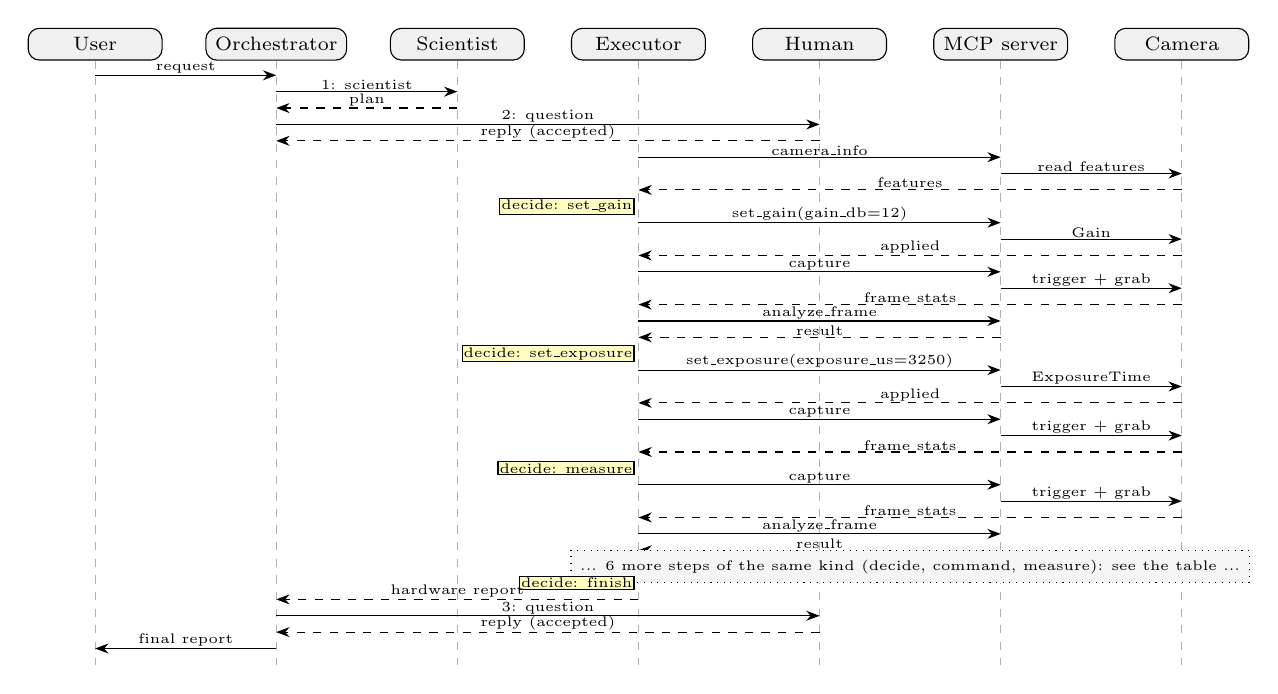
\begin{tikzpicture}[x=1cm,y=-0.208cm,font=\scriptsize,>=Stealth]
\node[draw,fill=gray!12,rounded corners,minimum width=17mm,align=center] at (0.00,-1.4) {User};
\draw[gray!60,dashed] (0.00,-0.4) -- (0.00,36.5);
\node[draw,fill=gray!12,rounded corners,minimum width=17mm,align=center] at (2.30,-1.4) {Orchestrator};
\draw[gray!60,dashed] (2.30,-0.4) -- (2.30,36.5);
\node[draw,fill=gray!12,rounded corners,minimum width=17mm,align=center] at (4.60,-1.4) {Scientist};
\draw[gray!60,dashed] (4.60,-0.4) -- (4.60,36.5);
\node[draw,fill=gray!12,rounded corners,minimum width=17mm,align=center] at (6.90,-1.4) {Executor};
\draw[gray!60,dashed] (6.90,-0.4) -- (6.90,36.5);
\node[draw,fill=gray!12,rounded corners,minimum width=17mm,align=center] at (9.20,-1.4) {Human};
\draw[gray!60,dashed] (9.20,-0.4) -- (9.20,36.5);
\node[draw,fill=gray!12,rounded corners,minimum width=17mm,align=center] at (11.50,-1.4) {MCP server};
\draw[gray!60,dashed] (11.50,-0.4) -- (11.50,36.5);
\node[draw,fill=gray!12,rounded corners,minimum width=17mm,align=center] at (13.80,-1.4) {Camera};
\draw[gray!60,dashed] (13.80,-0.4) -- (13.80,36.5);
\draw[->] (0.00,0.5) -- node[above,inner sep=0.5pt,font=\tiny] {request} (2.30,0.5);
\draw[->] (2.30,1.5) -- node[above,inner sep=0.5pt,font=\tiny] {1: scientist} (4.60,1.5);
\draw[->,dashed] (4.60,2.5) -- node[above,inner sep=0.5pt,font=\tiny] {plan} (2.30,2.5);
\draw[->] (2.30,3.5) -- node[above,inner sep=0.5pt,font=\tiny] {2: question} (9.20,3.5);
\draw[->,dashed] (9.20,4.5) -- node[above,inner sep=0.5pt,font=\tiny] {reply (accepted)} (2.30,4.5);
\draw[->] (6.90,5.5) -- node[above,inner sep=0.5pt,font=\tiny] {camera\_info} (11.50,5.5);
\draw[->] (11.50,6.5) -- node[above,inner sep=0.5pt,font=\tiny] {read features} (13.80,6.5);
\draw[->,dashed] (13.80,7.5) -- node[above,inner sep=0.5pt,font=\tiny] {features} (6.90,7.5);
\node[draw,fill=yellow!25,inner sep=0.6pt,font=\tiny,anchor=east] at (6.85,8.5) {decide: set\_gain};
\draw[->] (6.90,9.5) -- node[above,inner sep=0.5pt,font=\tiny] {set\_gain(gain\_db=12)} (11.50,9.5);
\draw[->] (11.50,10.5) -- node[above,inner sep=0.5pt,font=\tiny] {Gain} (13.80,10.5);
\draw[->,dashed] (13.80,11.5) -- node[above,inner sep=0.5pt,font=\tiny] {applied} (6.90,11.5);
\draw[->] (6.90,12.5) -- node[above,inner sep=0.5pt,font=\tiny] {capture} (11.50,12.5);
\draw[->] (11.50,13.5) -- node[above,inner sep=0.5pt,font=\tiny] {trigger + grab} (13.80,13.5);
\draw[->,dashed] (13.80,14.5) -- node[above,inner sep=0.5pt,font=\tiny] {frame stats} (6.90,14.5);
\draw[->] (6.90,15.5) -- node[above,inner sep=0.5pt,font=\tiny] {analyze\_frame} (11.50,15.5);
\draw[->,dashed] (11.50,16.5) -- node[above,inner sep=0.5pt,font=\tiny] {result} (6.90,16.5);
\node[draw,fill=yellow!25,inner sep=0.6pt,font=\tiny,anchor=east] at (6.85,17.5) {decide: set\_exposure};
\draw[->] (6.90,18.5) -- node[above,inner sep=0.5pt,font=\tiny] {set\_exposure(exposure\_us=3250)} (11.50,18.5);
\draw[->] (11.50,19.5) -- node[above,inner sep=0.5pt,font=\tiny] {ExposureTime} (13.80,19.5);
\draw[->,dashed] (13.80,20.5) -- node[above,inner sep=0.5pt,font=\tiny] {applied} (6.90,20.5);
\draw[->] (6.90,21.5) -- node[above,inner sep=0.5pt,font=\tiny] {capture} (11.50,21.5);
\draw[->] (11.50,22.5) -- node[above,inner sep=0.5pt,font=\tiny] {trigger + grab} (13.80,22.5);
\draw[->,dashed] (13.80,23.5) -- node[above,inner sep=0.5pt,font=\tiny] {frame stats} (6.90,23.5);
\node[draw,fill=yellow!25,inner sep=0.6pt,font=\tiny,anchor=east] at (6.85,24.5) {decide: measure};
\draw[->] (6.90,25.5) -- node[above,inner sep=0.5pt,font=\tiny] {capture} (11.50,25.5);
\draw[->] (11.50,26.5) -- node[above,inner sep=0.5pt,font=\tiny] {trigger + grab} (13.80,26.5);
\draw[->,dashed] (13.80,27.5) -- node[above,inner sep=0.5pt,font=\tiny] {frame stats} (6.90,27.5);
\draw[->] (6.90,28.5) -- node[above,inner sep=0.5pt,font=\tiny] {analyze\_frame} (11.50,28.5);
\draw[->,dashed] (11.50,29.5) -- node[above,inner sep=0.5pt,font=\tiny] {result} (6.90,29.5);
\node[draw,dotted,fill=gray!8,font=\tiny,minimum width=7.30cm] at (10.35,30.5) {... 6 more steps of the same kind (decide, command, measure): see the table ...};
\node[draw,fill=yellow!25,inner sep=0.6pt,font=\tiny,anchor=east] at (6.85,31.5) {decide: finish};
\draw[->,dashed] (6.90,32.5) -- node[above,inner sep=0.5pt,font=\tiny] {hardware report} (2.30,32.5);
\draw[->] (2.30,33.5) -- node[above,inner sep=0.5pt,font=\tiny] {3: question} (9.20,33.5);
\draw[->,dashed] (9.20,34.5) -- node[above,inner sep=0.5pt,font=\tiny] {reply (accepted)} (2.30,34.5);
\draw[->] (2.30,35.5) -- node[above,inner sep=0.5pt,font=\tiny] {final report} (0.00,35.5);
\end{tikzpicture}\end{center}

\subsection*{Use case 7 (no camera): focusing prediction at the Homework 2 settings, with the measured camera}
\textbf{Request:} \emph{Do not use the camera. The lab camera (Hikrobot MV-CS028-10UM) was measured in an earlier run: conversion gain 6.14 e-/DN, read noise 5.78 e-, full well at least 24766 e-. With the focusing tool, compare the focusing enhancement at the Homework 2 settings (macropixel 4, focus\_size 3, bg\_inner 6, bg\_outer 20, bg\_regions 8, iterations 40000, flips 4, remeasure true) for the bench's default camera and for this measured camera, with the bench signal level chosen so that the focus does not saturate this camera. Report both enhancements.}\\
Camera: not used in this run (simulated bench only); 3 orchestrator decisions, 0 hardware decisions, 0 MCP tool calls.
\\{\small\textbf{Focusing tool calls:} experiment 1: \{"macropixel": 4, "focus\_size": 3, "bg\_inner": 6, "bg\_outer": 20, "bg\_regions": 8, "iterations": 40000, "flips": 4, "flips\_...; experiment 2: \{"macropixel": 4, "focus\_size": 3, "bg\_inner": 6, "bg\_outer": 20, "bg\_regions": 8, "iterations": 40000, "flips": 4, "flips\_...; experiment 3: \{"macropixel": 4, "focus\_size": 3, "bg\_inner": 6, "bg\_outer": 20, "bg\_regions": 8, "iterations": 40000, "flips": 4, "flips\_...; experiment 4: \{"macropixel": 4, "focus\_size": 3, "bg\_inner": 6, "bg\_outer": 20, "bg\_regions": 8, "iterations": 40000, "flips": 4, "flips\_....}
\\\textbf{Verified result:} focusing tool (simulated bench), experiment 4: enhancement 30.63.
\par\smallskip\textbf{Sequence diagram} (as above; long hardware turns shortened).
\begin{center}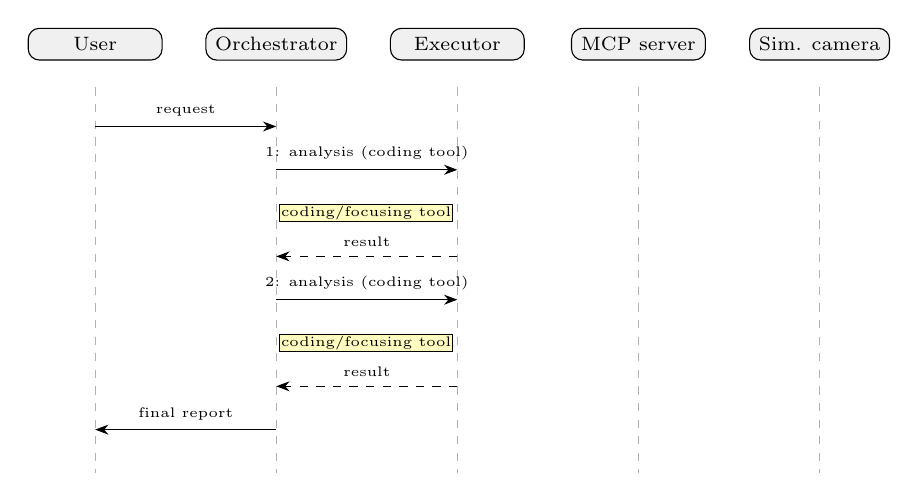
\begin{tikzpicture}[x=1cm,y=-0.550cm,font=\scriptsize,>=Stealth]
\node[draw,fill=gray!12,rounded corners,minimum width=17mm,align=center] at (0.00,-1.4) {User};
\draw[gray!60,dashed] (0.00,-0.4) -- (0.00,8.5);
\node[draw,fill=gray!12,rounded corners,minimum width=17mm,align=center] at (2.30,-1.4) {Orchestrator};
\draw[gray!60,dashed] (2.30,-0.4) -- (2.30,8.5);
\node[draw,fill=gray!12,rounded corners,minimum width=17mm,align=center] at (4.60,-1.4) {Executor};
\draw[gray!60,dashed] (4.60,-0.4) -- (4.60,8.5);
\node[draw,fill=gray!12,rounded corners,minimum width=17mm,align=center] at (6.90,-1.4) {MCP server};
\draw[gray!60,dashed] (6.90,-0.4) -- (6.90,8.5);
\node[draw,fill=gray!12,rounded corners,minimum width=17mm,align=center] at (9.20,-1.4) {Sim. camera};
\draw[gray!60,dashed] (9.20,-0.4) -- (9.20,8.5);
\draw[->] (0.00,0.5) -- node[above,font=\tiny] {request} (2.30,0.5);
\draw[->] (2.30,1.5) -- node[above,font=\tiny] {1: analysis (coding tool)} (4.60,1.5);
\node[draw,fill=yellow!25,inner sep=0.6pt,font=\tiny,anchor=east] at (4.55,2.5) {coding/focusing tool};
\draw[->,dashed] (4.60,3.5) -- node[above,font=\tiny] {result} (2.30,3.5);
\draw[->] (2.30,4.5) -- node[above,font=\tiny] {2: analysis (coding tool)} (4.60,4.5);
\node[draw,fill=yellow!25,inner sep=0.6pt,font=\tiny,anchor=east] at (4.55,5.5) {coding/focusing tool};
\draw[->,dashed] (4.60,6.5) -- node[above,font=\tiny] {result} (2.30,6.5);
\draw[->] (2.30,7.5) -- node[above,font=\tiny] {final report} (0.00,7.5);
\end{tikzpicture}\end{center}


\subsection*{Dry runs on the simulated camera}
Before the lab session the same system ran six requests on the simulated camera behind the same MCP server
(\texttt{--camera sim} or \texttt{sim-room}; runs \texttt{agent/runs/uc1}--\texttt{uc6}). Because the simulated camera's
true parameters are known, these runs check the method: the agent's photon-transfer measurements gave 2.30 and
2.41\,e$^-$/DN and 5.66 and 6.04\,e$^-$ read noise (true: 2.40\,e$^-$/DN and 6.0\,e$^-$), and in the room-light scene it
found the 100\,Hz flicker (22\,\% at 1\,ms, 0.27\,\% at 30\,ms).
\clearpage
%======================================================================
\section*{(g) Added after the deadline extension}
%======================================================================
The lab session showed that two camera settings decide whether a noise measurement is right: with the camera's default
8-bit ADC a Mono12 frame has only about 240 levels (steps of 16\,DN, larger than the read noise), and with the default
black level the dark level sits at 0\,DN and half of the dark noise is clipped. The connector fixed both at start-up.
They are now \textbf{tools the agent can use}, together with two more, so the MCP server has 13 tools (table in (b)):

\begin{center}\small
\begin{tabular}{@{}p{0.2\linewidth}p{0.26\linewidth}p{0.27\linewidth}p{0.2\linewidth}@{}}
\toprule
tool & what it does & lab camera (GenICam node) & simulated camera\\ \midrule
\texttt{set\_black\_level} & offset added before digitisation; returns the applied value &
  \texttt{BlackLevel} (integer; a larger value gives a lower dark level: 240 $\to$ 0\,DN, 180 $\to$ 62\,DN) &
  the dark level in DN\\
\texttt{set\_adc\_bit\_depth} & 8 or 12 bits of the ADC & \texttt{ADCBitDepth} (\texttt{Bits\_8}/\texttt{Bits\_12}),
  changed with the acquisition stopped & rounds to 256 levels of the 12-bit scale\\
\texttt{read\_temperature} & device temperature in $^\circ$C (dark current depends on it) & \texttt{DeviceTemperature} &
  warms from 38 to 41\,$^\circ$C in about 10 minutes\\
\texttt{save\_tiff} & a capture as a 16-bit multi-page TIFF for ImageJ/Fiji & on the server (Pillow) & the same\\
\bottomrule
\end{tabular}
\end{center}

The new settings are part of the camera interface (\texttt{camera/base.py}), so every connector offers them or refuses
them with a reason. A restarted server restores them from \texttt{calls.jsonl} like exposure and gain, every capture
reports them in its settings, and in the hardware turn \texttt{read\_temperature} and \texttt{save\_tiff} are commands
after which no frame is captured; the VERIFIED record of a hardware turn lists the temperatures read and the TIFF files.

\textbf{Packaging.} \texttt{hw3.py} is one entry point: \texttt{test} (all offline tests with a summary),
\texttt{check-camera} (the MVS SDK, then the plugged-in camera), \texttt{tools} (the server's tools as an MCP client sees
them), \texttt{run}, \texttt{live}, \texttt{demo}, and \texttt{mcp-config} (the entry that adds the camera server to any
MCP client, e.g.\ Claude Desktop). Every model call through the Claude Code CLI is now counted (calls, input and output
tokens, the CLI's cost estimate), and \texttt{model@low} lowers the model's thinking effort (36\,\% fewer output
tokens in a test). The MCP client always uses the Windows proactor event loop, so the camera server also starts inside
other programs, such as the web app of Homeworks~4/5.

\textbf{Tests} (\texttt{python hw3.py test}, simulated camera; all three suites pass). With the 8-bit ADC every value of a
dark frame is a multiple of $4095/255$ (16, 32, 48, 64\,DN, \dots); a black level of 100 gives a dark level of
100.0\,DN; the TIFF has one page per frame, equal to the frames; the device temperature reads 38.07\,$^\circ$C; and a
restarted server restores the 8-bit ADC, the black level of 100 and the gain of 6\,dB.

\textbf{Used by the agent.} In a run of the lab assistant of Homeworks~4/5 on the simulated camera (request: measure the
noise model and predict the focusing enhancement with it), the instrument team itself set the ADC to 12 bits and the
black level to 40 before its photon-transfer measurement, switched the light off with \texttt{set\_illumination} for 50
dark frames, and reported a conversion gain of 2.401\,e$^-$/DN (true value 2.40), a dark noise of 2.52\,DN and a full well
of at least 9737\,e$^-$ (true 10\,000\,e$^-$, not reached up to 30\,ms). It marked its read noise of 6.04\,e$^-$ (true
6.0\,e$^-$) as not verified because a cross-check failed; the optics team then predicted an enhancement of about 5.4 to
6.4 at 64 segments and 1000 iterations with this camera model.

\textbf{On the lab camera} the new connector functions use the same SDK calls as the connector's start-up, which ran at
the lab (\texttt{SetIntValueEx} for \texttt{BlackLevel}, \texttt{SetEnumValue} for \texttt{ADCBitDepth}), plus
\texttt{GetFloatValue} for \texttt{DeviceTemperature}; \texttt{tests/check\_real\_camera.py} now also checks them (black
level up and back, 8- and 12-bit frames, temperature). This check runs at the next lab session (18 October), before the
live demonstration of Homeworks~4/5.

\end{document}
